%%%%%%%%%%%%%%%%%%%%%%%%%%%%%%%%%%%%%%%%%%%%%%%%%%%%%%%%%%%%%%%%%%%%%%
% Source: Dave Richeson (divisbyzero.com), Dickinson College
% 
% A one-size-fits-all LaTeX cheat sheet. Kept to two pages, so it 
% can be printed (double-sided) on one piece of paper
% 
% Feel free to distribute this example, but please keep the referral
% to divisbyzero.com
% 
% If you're new to LaTeX, the wikibook is a great place to start:
% http://en.wikibooks.org/wiki/LaTeX
%%%%%%%%%%%%%%%%%%%%%%%%%%%%%%%%%%%%%%%%%%%%%%%%%%%%%%%%%%%%%%%%%%%%%%

\documentclass[10pt,landscape]{article}
\usepackage{amssymb,amsmath,amsthm,amsfonts}
\usepackage{multicol,multirow}
\usepackage{calc}
\usepackage{ifthen}
\usepackage{bm}
\usepackage[landscape]{geometry}
\usepackage[colorlinks=true,citecolor=blue,linkcolor=blue]{hyperref}
\usepackage{graphicx}
\usepackage{fixltx2e}
\graphicspath{{./images/}}

\ifthenelse{\lengthtest { \paperwidth = 11in}}
    { \geometry{top=0.1in,left=0.1in,right=0.1in,bottom=0.1in} }
	{\ifthenelse{ \lengthtest{ \paperwidth = 297mm}}
		{\geometry{top=0.1cm,left=0.1cm,right=0.1cm,bottom=0.1cm} }
		{\geometry{top=0.1cm,left=0.1cm,right=0.1cm,bottom=0.1cm} }
	}
\pagestyle{plain}
\makeatletter
\renewcommand{\section}{\@startsection{section}{1}{0mm}%
                                {-1ex plus -.5ex minus -.2ex}%
                                {0.5ex plus .2ex}%x
                                {\normalfont\large\bfseries}}
\renewcommand{\subsection}{\@startsection{subsection}{2}{0mm}%
                                {-1explus -.5ex minus -.2ex}%
                                {0.5ex plus .2ex}%
                                {\normalfont\normalsize\bfseries}}
\renewcommand{\subsubsection}{\@startsection{subsubsection}{3}{0mm}%
                                {-1ex plus -.5ex minus -.2ex}%
                                {1ex plus .2ex}%
                                {\normalfont\small\bfseries}}                       
\makeatother
\setcounter{secnumdepth}{0}
\setlength{\parindent}{0pt}
\setlength{\parskip}{0pt plus 0.5ex}
% -----------------------------------------------------------------------

\title{MA2101 Final Cheat Sheet}

\begin{document}

\raggedright
%\footnotesize
\scriptsize

\begin{center}
     \Large{\textbf{NUS MA2101 Final Cheat Sheet}} \\
\end{center}
\begin{multicols}{4}
\setlength{\premulticols}{1pt}
\setlength{\postmulticols}{1pt}
\setlength{\multicolsep}{1pt}
\setlength{\columnsep}{1pt}

\section{1: Vector Spaces}
% \subsection{Number Systems}
% $\mathbb{Z} = \{ 0, \pm 1, \pm 2, \cdots \}$ is the set of \textit{integers}.

% $\mathbb{Q} = \{ \frac{p}{q}: p, q \in \mathbb{Z}, q \neq 0 \} $ is the set of \textit{rational numbers}.

% $\mathbb{R}$ denotes the set of \textit{real numbers}.

% $\mathbb{C} = \{ x + iy: x, y \in \mathbb{R} \} $ is the set of \textit{complex numbers}.

% $\mathbb{Z} \subset \mathbb{Q} \subset \mathbb{R} \subset \mathbb{C}$

% \subsection{Systems of Linear Equations}
% \textbf{EROs}
% $cR_j$ - multiply row $j$ by a nonzero scalar $c$

% $cR_j + R_k$ - replace row $k$ by row $k$ plus $c$ times row $j$

% $R_j \leftrightarrow R_k$ - interchange row $j$ and row $k$

% \subsection{Field}
% \textbf{Definition.} A \textit{field} $\mathbb{F, +, \times}$ is a set $\mathbb{F}$ together with two binary operations $+$ and $\times$ called \textit{addition} and \textit{multiplication} respectively satisfying the following axioms:

% \textbf{(A1)} (Closure for addition) For all $x, y \in \mathbb{F}, x + y \in \mathbb{F}$.

% \textbf{(A2)} (Addition is commutative) $x + y = y + x$ for all $x, y \in \mathbb{F}$.

% \textbf{(A3)} (Addition is associative) $(x + y) + z = x + (y + z)$ for all $x, y, z \in \mathbb{F}$.

% \textbf{(A4)} (Additive identity) There exists $0 \in \mathbb{F}$ st for all $x \in \mathbb{F}$, $x + 0 = x$.
% Note that (A4) defines $0$.

% \textbf{(A5)} (Additive inverse) For every $x \in \mathbb{F}$ there exists $y \in \mathbb{F}$ (y depends on x) such that $x + y = 0.$ We denote $y$ by $-x$.

% \textbf{(M1)} (Closure for multiplication) For all $x, y \in \mathbb{F}, x \times y \in \mathbb{F}$.

% \textbf{(M2)} (Multiplication is commutative) $x \times y = y \times x$ for all $x, y \in \mathbb{F}$.

% \textbf{(M3)} (Multiplication is associative) $(x \times y) \times z = x \times (y \times z)$ for all $x, y, z \in \mathbb{F}$.

% \textbf{(M4)} (Multiplicative identity) There exists $1 = 1_{\mathbb{F}} \in \mathbb{F}, 1 \neq 0$ such that for all $x \in \mathbb{F}$, $1 \times x = x$.
% Note that (M4) defines $1$.

% \textbf{(M5)} (Multiplicative inverse) For every nonzero $x \in \mathbb{F}$ there exists $y \in \mathbb{F}$ ($y$ depends on $x$) such that $x \times y = 1$. We call $y$ the multiplicative inverse of $x$ and we denote $y$ by $x^{-1}$.

% \textbf{(D)} (Distributive Law) $x \times (y + z) = (x \times y) + (x \times z)$ for all $x, y, z \in \mathbb{F}$.

% \textbf{Remark.} Axioms (A1)-(A5) says that $(\mathbb{F}, +)$ forms a \textit{commutative group}, and axioms (M1)-(M5) says that $(\mathbb{F} - \{ 0 \}, \times)$ forms another \textit{commutative group}. Axiom (D) connect the two group structures.

% \textbf{Remarks.} A field which contains only finitely many elements is called a finite field. It turns out that the number of elements in a finite field is of the form $q = p^m$ where $p$ is prime and $m$ a positive integer. For each such $q$, there is exactly one field (up to isomorphism) with $q$ elements. So we can safely denote this field by $\mathbb{F}_q$.

% \textbf{Example.} The sets $\mathbb{R, C, Q}$ with the usual addition and multiplication is a field. However, $\mathbb{Z}$ is not a field.

% \textbf{Theorem 1.3.1.} Let $\mathbb{F}$ be a field.

% If $a \in \mathbb{F}$, then $0a = 0$.

% If $a \in \mathbb{F}$, then $(-1)a = -a$.

% If $a, b \in \mathbb{F}$ and $ab = 0$, then \textit{either} $a = 0$ or $b = 0$.

% \textbf{Definition.} Let $\mathbb{F}$ be a field and $1_{\mathbb{F}}$ be its multiplicative identity. For each positive integer $n$, let $n1_{\mathbb{F}} = \overbrace{1_{\mathbb{F}} + 1_{\mathbb{F}} + \cdots + 1_{\mathbb{F}}}^n$.

% If $n1_{\mathbb{F}} \neq 0$ for all positive integers $n$, then we say $\mathbb{F}$ is of \textit{characteristic} 0. For example, the fields $\mathbb{Q, R, C}$.

% If $n1_{\mathbb{F}} = 0$ for some positive integer $n$, and $p$ is the smallest positive integer such that $p1_{\mathbb{F}} = 0$, then we say $\mathbb{F}$ has \textit{characteristic p}. For example, the field $\mathbb{F}_2 = \{ 0, 1 \}$ has characteristic 2.

\subsection{Matrices}
\textbf{Matrix Multiplication} 

% If $A = (a_{ij}) \in M_{mn}(\mathbb{F})$ and $B = (b_{ij}) \in M_{nr}(\mathbb{F})$, then $AB = (c_{ij}) \in M_{mr}(\mathbb{F})$ where

% $$
% c_{ij} = \sum^n_{k = 1} a_{ik} b_{kj}
% $$

(i) (element) Let $(AB) = (c_{ij})$. $c_{ij} = \sum^n_{k = 1} a_{ik} b_{kj}$.

(ii) (matrix multiplied by column) $A_{nn}c_{n1} = (\mathbf{a_1}| \cdots | \mathbf{a_n})(c_1 \cdots c_n)^T = c_1 \mathbf{a_1} + \cdots + c_n \mathbf{a_n}$.

(iii) (matrix multiplied by matrix) $AB = A (\mathbf{b_1} | \cdots | \mathbf{b_n}) = (A\mathbf{b_1} | \cdots | A\mathbf{b_n})$

% \textbf{Definition.} Let $\mathbb{F}$ be a field and let $M_{mn}(\mathbb{F})$ be the set of all $m \times n$ matrices $A$ with entries taken from $\mathbb{F}$

\textbf{Theorem 1.4.1. (Associative Law)} If $A, B, C$ are matrices over the field $\mathbb{F}$ st products BC and $A(BC)$ are defined, then $A(BC) = (AB)C$.

\textbf{Theorem (Distributive Law)} If $A, B, C$ are matrices of respective sizes $m \times n, n \times p, n \times p$, then 

$$
A(B + C) = AB + AC
$$

% \textbf{Homogeneous System.} Let $\mathbb{F}$ be a field. Consider the problem of finding $x_1, \cdots, x_n \in \mathbb{F}$ st

% $$
% \begin{aligned}
% a_{11}& x_{1}+a_{12} x_{2}+\cdots+a_{1 n} x_{n} &=0 \\
% a_{21}& x_{1}+a_{22} x_{2}+\cdots+a_{2 n} x_{n} &=0 \\
% \vdots &  & \vdots \\
% a_{m 1}& x_{1}+a_{m 2} x_{2}+\cdots+a_{m n} x_{n} &=0
% \end{aligned}
% $$

% where $a_{ij} \in \mathbb{F}, \enskip \forall 1 \leq i \leq m, 1 \leq j \leq n$. We call the above a \textbf{homogeneous system of $m$ linear equations in $n$ variables over the field $\mathbb{F}$}. It has at least the \textbf{trivial solution}.

% \textbf{Linear Combination.} If $c_1, \cdots, c_m \in \mathbb{F}$, then the equation

% \begin{equation*}
%     \begin{aligned}
%     & c_{1}\left(a_{11} x_{1}+a_{12} x_{2}+\cdots+a_{1 n} x_{n}\right)+ \\
%     & \cdots+c_{m}\left(a_{m 1} x_{1}+a_{m 2} x_{2}+\cdots+a_{m n} x_{n}\right)=0
%     \end{aligned}
% \end{equation*}

% is called a linear combination of the homogenous system of linear equations.

% \textbf{Definition.} Two homogenous systems of linear equations are \textbf{equivalent} if each equation in one system is a linear combination of the equations in the other system.

% \textbf{Theorem 1.4.2.} Two equivalent homogenous linear systems of linear equations have exactly the same solutions.

% \textbf{Definition.} If $A, B \in M_{mn}(\mathbb{F)}$, then we say $B$ is \textbf{row-equivalent} to $A$ if $B$ can be obtained from $A$ by a finite sequence of elementary row operations.

% \textbf{Theorem 1.4.3.} If $A, B \in M_{mn}(\mathbb{F})$ and $B$ is row equivalent to $A$, then the homogenous linear systems $A\bm{x} = 0$ and $B\bm{x} = 0$ are equivalent. By Theorem 1.4.2, they have the same solutions.

% For the sequence of EROs from A to B, each row of B is a linear combination of the rows of A. Inversing this sequence of EROs from B to A, each row of A is a linear combination of the row of B. Thus A and B are equivalent.

% \textbf{Theorem 1.4.4.} Every $m \times n$ matrix $A$ over $\mathbb{F}$ is row equivalent to a matrix $B$ in RREF.

% \textbf{Theorem 1.4.5.} If $m < n$ and $A \in M_{mn}(\mathbb{F})$, then the homogenous system of linear equations $A\bm{x} = 0$ has a nontrivial solution.

\subsection{Determinant}
% \textbf{Definition} Let $A \in M_n(\mathbb{F})$ be a square matrix. We say that $A$ is \textit{invertible} if there is a matrix $B \in M_n(\mathbb{F})$ such that $AB = BA = I$. In this case, $A^{-1} = B$.

% \textbf{Theorem 1.5.1.} A \textit{square matrix} $A \in M_n(\mathbb{F})$ is \textit{invertible iff} $detA \neq 0$.

% \textbf{Definition} Let $U$ and $V$ be vector spaces over a field $K$. A mapping $A: U \mapsto V$ is linear 

% $$ A(\alpha \mathbf{x} + \beta \mathbf{y}) = \alpha A \mathbf{x} + \beta A \mathbf{y} $$

% $\forall \mathbf{x, y} \in U, \forall \alpha, \beta \in K$. Linear operators are morphisms between vector spaces.

\textbf{Definition} A function $D: M_n(\mathbb{F}) \mapsto \mathbb{F}$ is called a \textbf{determinant function} if it has the following properties:

(D1) It is \textit{multilinear.} We regard $D$ as a function on $n-tuples$ of column vectors: $D(X) = D(X_1, \cdots, X_n)$ where $X = (x_{ij})$ and $X_1, \cdots, X_n$ are the columns of X. Then $D$ is a \textbf{linear function} of each column when the other columns are held fixed, that is, for each $1 \leq j \leq n, \alpha, \beta \in \mathbb{F}$ and column vectors $X_1, \cdots, X_{j-1}, X_{j+1}, \cdots, X_n, \mathbf{u}, \mathbf{v}$,
\begin{equation*}
    \begin{aligned}
    &D(X_1, \cdots, X_{j-1}, \alpha \mathbf{u} + \beta \mathbf{v}, X_{j+1}, \cdots, X_n) \\
    &= \alpha D(X_1, \cdots, X_{j-1}, \mathbf{u} , X_{j+1}, \cdots, X_n) \\
    &+ \beta D(X_1, \cdots, X_{j-1}, \mathbf{v} , X_{j+1}, \cdots, X_n)
    \end{aligned}
\end{equation*}

% \textbf{Remark} If $\mathbf{v} = \mathbf{0}$, then 

% \begin{equation*}
%     \begin{aligned}
%     &D(X_1, \cdots, X_{j-1}, \alpha \mathbf{u}, X_{j+1}, \cdots, X_n) \\
%     &= \alpha D(X_1, \cdots, X_{j-1}, \mathbf{u} , X_{j+1}, \cdots, X_n)
%     \end{aligned}
% \end{equation*}

(D2) It is \textit{alternating}. This means that if $X$ has two equal columns, then $D(X) = 0$.

(D3) If $I$ is the $n \times n$ identity matrix, then

$$
D(I) = 1
$$

\textbf{Theorem 1.5.2.} Let the function $D: M_n(\mathbb{F}) \mapsto \mathbb{F}$ be multilinear and alternating. If $X \in M_n(\mathbb{F})$ and $X'$ is the matrix obtained from $X$ by interchanging two columns then

$$
D(X') = -D(X)
$$

% \textbf{Example.} The function $D: M_2(\mathbb{F}) \mapsto \mathbb{F}$ given by 

% $$
% D \begin{pmatrix}
% x_{11} & x_{12} \\
% x_{21} & x_{22}
% \end{pmatrix}
% = x_{11}x_{22} - x_{21}x_{12}
% $$

% This example serves as base case for Theorem 1.5.3.

% \textbf{Theorem 1.5.3.} Let $D: M_{n-1}(\mathbb{F}) \mapsto \mathbb{F}$ be a determinant function on $M_{n-1}(\mathbb{F})$ and $1 \leq i \leq n$. Define $E: M_n(\mathbb{F}) \mapsto \mathbb{F}$ by 

% $$
% E(X) = \sum^n_{j=1} (-1)^{i+j}x_{ij}D(\Tilde{X}_{ij}), \quad X \in M_n(\mathbb{F})
% $$

% Then E is a determinant function on $M_n(\mathbb{F})$. Note that $i$ is chosen.

% \textbf{Corollary 1.5.4.} For each positive integer $n$, there is at least one determinant function on $M_n(\mathbb{F})$.

% \textbf{Definition.} Let $\sigma = (\sigma_1, \cdots, \sigma_n)$ be a permutation. Let $m$ denote the number of interchanges of pairs $(i,j)$ to pass from $(\sigma_1, \cdots, \sigma_n)$ to $(1, 2, \cdots, n)$.

% $$
% sgn(\sigma) = (-1)^m
% $$

% \textbf{Theorem 1.5.5.} For each positive integer $n$, there is exactly one determinant function on $M_n(\mathbb{F})$ denoted by 

% $$
% det:M_n(\mathbb{F}) \mapsto \mathbb{F}.
% $$

% It is given by 

% \begin{equation*}
%     \begin{aligned}
%     % &\operatorname{det} A=\sum_{\sigma \in S_{n}} \operatorname{sgn}(\sigma) a_{\sigma 1,1} a_{\sigma 2,2} \cdots a_{\sigma n, n} \\
%     &\operatorname{det} A=\sum_{\sigma \in S_{n}} \operatorname{sgn}(\sigma) \prod_{i=1}^n a_{\sigma i, i} \\
%     &A=\left(a_{i j}\right) \in \mathbf{M}_{n}(\mathbb{F})
%     \end{aligned}
% \end{equation*}

% \textbf{Theorem 1.5.6.} If $D : M_n(\mathbb{F}) \mapsto \mathbb{F}$ is multilinear and alternating, then for $A \in M_n(\mathbb{F})$,

% $$
% D(A) = (\operatorname{det}A)D(I)
% $$

% Note that $D$ can be a user-defined function that's not necessary the determinant function.

\textbf{Theorem 1.5.7. (Cofactor expansion along row $i$)}. If $A = (a_{ij}) \in M_n(\mathbb{F})$ and $1 \leq i \leq n$, then 

$$
\operatorname{det} A = \sum^n_{j = 1}(-1)^{i+j}a_{ij}\operatorname{det}\Tilde{A}_{ij}
$$

Note that row $i$ is fixed and $i$ need not necessarily be 1. Differs from theorem 1.5.3 in that it uses theorem 1.5.5 to replace the determinant function with the function's evaluation. 

\textbf{Corollary.} Let $A = (a_{ij}) \in M_n(\mathbb{F})$ be an upper or lower triangular matrix. Then

$$
\operatorname{det}(A) = \prod^n_{k=1} a_{kk} 
$$

% Proof. Expand with respect to the first row, which gives only one nonzero term, and then continue in the same way (for the upper triangular case expand with respect to the last row).

\textbf{Theorem 1.5.8.} If $A \in M_r(\mathbb{F}), B \in M_{rs}(\mathbb{F})$ and $C \in M_s(\mathbb{F})$, then 
$$
\operatorname{det} 
\begin{pmatrix}
A & B \\
0 & C 
\end{pmatrix} = (\operatorname{det}A)(\operatorname{det}C)
$$
\textbf{Theorem 1.5.9.} If $A, B \in M_n(\mathbb{F}), then$
$$
\operatorname{det}(AB) = \operatorname{det}A\operatorname{det}B
$$
\textbf{Theorem 1.5.10.} If $A \in M_n(\mathbb{F})$ and $A^t$ is its transpose, then
$$
\operatorname{det}A^t = \operatorname{det} A
$$
\textbf{Theorem 1.5.11. (Cofactor expansion along column $j$)} If $A = (a_{ij}) \in M_n(\mathbb{F})$ and $1 \leq j \leq n$, then 
$$
\operatorname{det} A = \sum^n_{i = 1}(-1)^{i+j}a_{ij} \operatorname{det}\Tilde{A}_{ij}
$$
Note that column $j$ is fixed and $j$ need not necessarily be 1.

% \subsection{General vector spaces}
% % \textbf{Definition} A \textit{vector space} consists of the following:

% % (i) a field $\mathbb{F}$ of scalars;

% % (ii) a nonempty set \textit{V} of objects, called vectors;

% % (iii) a rule called \textit{vector addition} such that for each pair of vectors $\mathbf{u}$ and $\mathbf{v}$ in \textit{V}, there is a unique vector $\mathbf{u} + \mathbf{v} \in V$. 

% % (iv) a rule called \textit{scalar multiplication} such that for each scalar $k \in \mathbb{F}$ and each vector $\mathbf{u} \in V$, there is a unique vector $k \mathbf{u}$ in $V$.

% \textbf{Definition.} In addition, these rules satisfy the following axioms:

% \textbf{(A1)} $V$ is closed under vector addition, i.e. $\forall \mathbf{v}, \mathbf{w} \in V, \mathbf{v} + \mathbf{w} \in V$.

% \textbf{(A2)} Vector addition is commutative, that is, for all $\mathbf{v, w} \in V,$

% $$
% \mathbf{v} + \mathbf{w} = \mathbf{w} + \mathbf{v}
% $$

% \textbf{(A3)} Vector addition is associative, i.e. $\forall \mathbf{u, v, w} \in V$,

% $$
% \mathbf{u} + (\mathbf{v} + \mathbf{w}) = (\mathbf{u} + \mathbf{v}) + \mathbf{w}
% $$

% \textbf{(A4)} $V$ has a unique vector $\mathbf{0}$, called the \textit{zero vector}, such that $\forall \mathbf{v} \in V$,

% $$
% \mathbf{v} + \mathbf{0} = \mathbf{v}
% $$

% \textbf{(A5)} For every vector $\mathbf{v}$, there is a vector $\mathbf{-v}$ in $V$, called the \textit{negative} of $\mathbf{v}$, such that 

% $$
% \mathbf{v} + \mathbf{-v} = \mathbf{0}
% $$

% \textbf{(S1)} $V$ is closed under scalar multiplication, i.e. $\forall k \in \mathbb{F}, \mathbf{v} \in V, k \mathbf{v} \in V$.

% \textbf{(S2)} $\forall k, l \in \mathbb{F}$ and $\mathbf{v} \in V$ we have

% $$
% (kl)\mathbf{v} = k(l\mathbf{v})
% $$

% \textbf{(S3)} $\forall \mathbf{v} \in V, 1\mathbf{v} = \mathbf{v}$. Note that 1 is a scalar, not a vector.

% \textbf{(D1)-(D2) Distributive Laws.}  For $k, l \in \mathbb{F}, \mathbf{v, w} \in V$ we have 

% \begin{align*}
%     &\text{(D1)} \quad k(\mathbf{v} + \mathbf{w}) = (k \mathbf{v}) + (k \mathbf{w}) \\    
%     &\text{(D2)} \quad (k + l)\mathbf{v} = (k\mathbf{v}) + (l\mathbf{v})
% \end{align*}

% % \textbf{Definition} 

% % (i) A \textit{polynomial} with coefficient in a field $\mathbb{F}$ is an expression of the form

% % $$
% % f(x) = a_0 +a_1x + \cdots + a_n x^n
% % $$

% % where $n$ is a nonnegative integer and $a_0, a_1, \cdots, a_n \in \mathbb{F}$. We also called $a_k$ the coefficient of $x^k$.

% % (ii) Two polynomials are called \textit{equal} if for each $k$ their coefficients of $x^k$ are equal.

% % (iii) The \textbf{zero polynomial} is the polynomial $p_0(x)$ such that all its coefficients are 0, that is $p_0(x) = 0 + 0x + \cdots + 0x^n$.

% \textbf{Theorem 1.7.1.} Let $V$ be a vector space over $\mathbb{F}, \mathbf{v} \in V$ and $k \in \mathbb{F}$. Then

% (i) $0\mathbf{v} = \mathbf{0}$

% (ii) $k\mathbf{0} = \mathbf{0}$

% (iii) $(-1)\mathbf{v} = \mathbf{-v}$

% (iv) if $k\mathbf{v} = \mathbf{0}$, then either $k = 0$ or $\mathbf{v = 0}$

% \subsection{Subspaces}
% \textbf{Theorem 1.8.1.} Let $V$ be a vector space over a field $\mathbb{F}$ and $W$ a \textbf{nonempty} subset of $V$. Then $W$ is a subspace of $V$ iff for any $\mathbf{u, v} \in W$ and any $\alpha, \beta \in \mathbb{F}$, we have $\alpha \mathbf{u} + \beta \mathbf{v} \in W$. Remember to check for nonempty subset!

% \textbf{Remarks} Note that subspaces are vector spaces, the only special thing about them is that they sit inside some bigger vector spaces and use the same operations as the big spaces. So Theorem 1.8.1 provides us with many new examples of vector spaces.

% \textbf{Definition} Let $f(x)$ be a nonzero polynomial with coefficients in $\mathbb{F}$. We say that $f(x)$ has degree $m$ if $f$ is of the form
% $$
% f(x) = a_0 + a_1x + \cdots + a_mx^m
% $$
% with $a_m \neq 0$. In this case, we write
% $$
% deg(f(x)) = m
% $$
% In particular, if $a_0 \neq 0$, the degree of the constant polynomial $f(x) = a_0$ is 0.

% \textbf{Definition} The degree of the zero polynomial is defined to be -1.

% \textbf{Notation} Let $P_n(\mathbb{F})$ be the set of all polynomials with coefficients in $\mathbb{F}$ of degree less than or equal $n$, that is,

% $$
% P_n(\mathbb{F}) = \{ a_0 + a_1x + \cdots + a_nx^n \enskip : \enskip a_0, a_1, \cdots, a_n \in \mathbb{F} \}
% $$

% $\mathcal{F}(\mathbb{R}, \mathbb{R})$: set of all real-valued functions on $\mathbb{R}$. That is, $\mathcal{F}: \mathbb{R} \mapsto \mathbb{R}$. The following spaces are subspaces of $\mathcal{F}(\mathbb{R}, \mathbb{R})$:

% $C(\mathbb{R})$: the space of all real-valued continuous functions on $\mathbb{R}$

% $C^1(\mathbb{R})$: the space of all real-valued continuously differentiable functions on $\mathbb{R}$

% $C^{\infty}(\mathbb{R}):$ the space of all real-valued continuously infinitely differentiable functions (or smooth functions) on $\mathbb{R}$.

% \textbf{Lemma 1.8.2.} Let $V$ be a vector space and $W_1, W_2$ be two subspaces of $V$. Define
% $$
% W_1 + W_2 = \{ \mathbf{w_1} + \mathbf{w_2}: \mathbf{w_1} \in W_1, \mathbf{w_2} \in W_2 \}
% $$
% Then $W_1 + W_2$ is a subspace of $V$, called the sum of $W_1$ and $W_2$.

% \subsection{Linear Combinations}

% \textbf{Definition} Let $V$ be a vector space over $\mathbb{F}$ and $S = \{ \mathbf{v}_1, \cdots, \mathbf{v}_r \}$ a nonempty finite set of vectors in $V$.

% (i) A vector $\mathbf{u}$ of the form 

% $$
% \mathbf{u} = \alpha_1 \mathbf{v}_1 + \alpha_2 \mathbf{v}_2 + \cdots + \alpha_r \mathbf{v}_r
% $$

% where $\alpha_1, \alpha_2, \cdots, \alpha_r \in \mathbb{F}$ is called a \textit{linear combination} of $\mathbf{v}_1, \cdots, \mathbf{v}_r$.

% (ii) The \textbf{span} of $S$ is the set

% $$
% Span(S) = \{ \alpha_1 \mathbf{v}_1 + \alpha_2 \mathbf{v}_2 + \cdots + \alpha_r \mathbf{v}_r : a_1, \cdots, a_r \in \mathbb{F} \}
% $$

% of all linear combination of $\mathbf{v}_1, \cdots, \mathbf{v}_r$.

% (iii) We also define $Span(\emptyset) = \{ \mathbf{0} \}$.

\textbf{Theorem 1.9.1.} Let $V$ be a vector space over $\mathbb{F}$ and $S$ a finite subset of vectors in $V$. Then:

(i) $Span(S)$ is a subspace of $V$

(ii) If $W$ is a subspace of $V$ and $S \subseteq W$ then $Span(S) \subseteq W$.

% \textbf{Remarks} Part (ii) implies that $Span(S)$ is the smallest subspace containing $S$.

% \textbf{Definition} If $W$ is a subspace of a vector space and $W = Span(S)$ where $S$ is a finite subset of $V$, then we say that $W$ is \textbf{spanned} by $S$. We also say that $S$ is a \textbf{spanning set} for $W$.

% \textbf{Example (Row and column space)} Let $A \in M_{mn}(\mathbb{F})$. 

% The subspace $Span\{ \mathbf{r}_1, \cdots, \mathbf{r}_m \}$ of $\mathbb{F}^n$ is called the \textit{row space} of $A$. 

% The subspace $Span\{ \mathbf{c}_1, \cdots, \mathbf{c}_n \}$ of $\mathbb{F}^m$ is called the \textit{column space} of $A$.

% \textbf{Definition} Let $V$ be a vector space over $\mathbb{F}$ and $S$ a nonempty subset of $V$. Then $Span(S)$ is the set of all linear combinations of the form $\alpha_1 \mathbf{v}_1 + \alpha_2 \mathbf{v}_2 + \cdots + \alpha_r \mathbf{v}_r$ with $\mathbf{v}_1, \cdots, \mathbf{v}_r \in S$ and $\alpha_1, \cdots, \alpha_r \in \mathbb{F}$.

% \subsection{Linear Dependence}

% \textbf{Definition} We say that the vectors $\mathbf{v}_1, \cdots, \mathbf{v}_r$ of $V$ are \textit{linearly dependent} (or the set $\{ \mathbf{v}_1, \cdots, \mathbf{v}_r \}$ is linearly dependent) if there exist scalars $c_1, \cdots, c_r \in \mathbb{F}$, \textit{not all of which are 0}, such that 

% $$
% c_1 \mathbf{v}_1 + c_2 \mathbf{v}_2 + \cdots + c_r \mathbf{v}_r = \mathbf{0}
% $$

% \textbf{Definition} We say that the vectors $\mathbf{v}_1, \cdots, \mathbf{v}_r$ of $V$ are \textit{linearly independent} (or the set $\{ \mathbf{v}_1, \cdots, \mathbf{v}_r \}$ is linearly independent) if they are not linearly dependent, that is, the only solution to the equation

% $$
% x_1 \mathbf{v}_1 + x_2 \mathbf{v}_2 + \cdots + x_r \mathbf{v}_r = \mathbf{0}
% $$

% is $x_1 = x_2 = \cdots = x_r = 0$.

% \textbf{Observations}

% (i) Any finite set containing the zero vector $\mathbf{0}$ is linearly dependent.

% (ii) If $\mathbf{v}$ is a nonzero vector in $V$, then the set $\{ \mathbf{v} \}$ is linearly independent.

% (iii) Two nonzero vectors $\mathbf{u}$ and $\mathbf{v}$ are linearly dependent iff one is a scalar multiple of the other.

% (iv) If a subset $\{ \mathbf{v}_1, \cdots, \mathbf{v}_r \}$ of $V$ is linearly dependent, then so is any finite subset of $V$ containing $\{ \mathbf{v}_1, \cdots, \mathbf{v}_r \}$.

% (v) If $S = \{ \mathbf{v}_1, \cdots, \mathbf{v}_r \} $ is linearly independent, then every subset of $S$ is linearly independent.

% \textbf{Definition} Let S be a subset of a vector space. (We do not assume $S$ is finite).

% We say that $S$ is \textit{linearly dependent} if $S$ has a finite subset which is linearly dependent.

% We say that $S$ is \textit{linearly independent} if it is not linearly dependent. Equivalently, $S$ is linearly independent if every finite subset of $S$ is linearly independent.

% The empty set $\emptyset$ is linearly independent.

% \textbf{Remarks}

% (i) Theorem 1.9.1 also holds when $S$ is an \textit{infinite} subset of $V$

% (ii) If $W$ is a subspace of a vector space $V$, then $W = Span(W)$. So every subspace has a spanning set.

% \textbf{Theorem 1.10.1.} If a subspace $W$ of a vector space is spanned by $S = \{ \mathbf{v}_1, \cdots, \mathbf{v}_r \}$ and $S$ is linearly dependent, then there is a vector $\mathbf{v}_i$ in $S$ such that 

% $$
% W = Span(S \backslash \{ \mathbf{v}_i \} )
% $$

% \textbf{Remarks} T1.10.1 says that a linearly dependent spanning set contains redundant vectors and suggests that the smallest spanning set should be one which is linearly independent.

% \subsection{Basis and Dimension}

% \textbf{Definition} A subset $\mathcal{B}$ of a vector space $V$ is called a \textit{basis} for $V$ if:

% (i) $\mathcal{B}$ spans $V$, and

% (ii) $\mathcal{B}$ is linearly independent.

% \textbf{Definition}

% (i) If a vector space $V$ has a finite basis, that is, a basis which consists of finitely many vectors, then we say $V$ is \textit{finite-dimensional}.

% (ii) A vector space which is not finite dimensional is called \textit{infinite-dimensional}.

% \textbf{Theorem 1.11.1} Let $\mathcal{B} = \{ \mathbf{v}_1, \cdots, \mathbf{v}_n \} $ be a basis for the vector space $V$. Then every vector $\textbf{v} \in V$ can be expressed in the form

% $$
% \mathbf{v} = \alpha_1 \mathbf{v}_1 + \alpha_2 \mathbf{v}_2 + \cdots + \alpha_n \mathbf{v}_n
% $$

% in exactly one way.

% \textbf{Theorem 1.11.2.} Suppose that a vector space $V$ has a finite spanning set $S$. Then any subset $L$ of $V$ with $|L| > |S|$ is linearly dependent.

% \textbf{Corollary 1.11.3.} If a vector space $V$ is spanned by a finite set $S$ and $L$ is linearly independent subset of $V$, then 

% $$
% |L| \leq |S|
% $$

% \textbf{Remarks} Corollary 1.11.3 says that a linearly independent set cannot contain more elements than a spanning set.

% \textbf{Theorem 1.11.4.} If $V$ is a finite dimensional vector space, then every basis of $V$ is finite and has the same number of elements.

% \textbf{Definition} Let $V$ be a finite dimensional vector space. The \textit{dimension} of $V$, denoted by $\dim V$, is the number of elements in a basis of $V$.

% \textbf{Theorem 1.11.5.} Suppose $\dim V = n$.

% (i) Any subset $S$ of $V$ which contains more than $n$ elements is linearly dependent.

% (ii) No subset of $V$ with less than $n$ elements spans $V$.

% \textbf{Theorem 1.11.6.} Let $\{ \mathbf{v}_1, \cdots, \mathbf{v}_m \}$ be a linearly independent subset of a vector space $V$. If $\mathbf{w}$ is a vector in $V$ such that

% $$
% \mathbf{w} \notin Span\{\mathbf{v}_1, \cdots, \mathbf{v}_m\},
% $$

% then the set

% $$
% \{ \mathbf{v}_1, \cdots, \mathbf{v}_m, w \}
% $$

% is linearly independent.

% \textbf{Corollary 1.11.7.} Suppose $\dim V = n$ and $S = \{ \mathbf{v}_1, \cdots, \mathbf{v}_n \}$ is a set of $n$ vectors in $V$.

% (i) If $S$ is linearly independent, then $S$ is a basis for $V$.

% (ii) If $S$ spans $V$, then $S$ is a basis for $V$.

% \textbf{Remarks} Corollary 1.11.7. says if you have the right number of vectors, then you only need to check one condition of a basis.

\subsection{Direct sum of subspaces}

% \textbf{Definition} Let $W_1$ and $W_2$ be subspaces of the vector space $V$. We say that the subspace $W_1 + W_2$ is the \textit{direct sum} of $W_1$ and $W_2$ if every vector $\mathbf{v} \in W_1 + W_2$ can be expressed \textbf{uniquely} as a sum

% $$
% \mathbf{v} = \mathbf{w}_1 + \mathbf{w}_2
% $$

% with $\mathbf{w}_1 \in W_1$ and $\mathbf{w}_2 \in W_2$. In this case, we shall denote $W_1 + W_2$ by $W_1 \oplus W_2$.

% \textbf{Theorem 1.13.1.} Let $W_1$ and $W_2$ be subspaces of the vector space $V$. Then the subspace $W_1 + W_2$ of $V$ is a direct sum of $W_1$ and $W_2$ iff $W_1 \cap W_2 = \{ \mathbf{0} \}$.

% \textbf{Definition} Let $V$ be a vector space and $W_1, \cdots, W_k$ are subspaces of $V$. Recall that $W_1 + W_2 + \cdots + W_k$ is the subspace of $V$ defined as 

% $$
% \begin{aligned}
% &W_1 + W_2 + \cdots + W_k = \\
% &\{ \mathbf{w}_1 + \mathbf{w}_2 + \cdots + \mathbf{w}_k : \mathbf{w}_i \in W_i, \forall 1 \leq i \leq k \}
% \end{aligned}
% $$

% We say that the subspace $W_1 + W_2 + \cdots + W_k$ is the \textit{direct sum} of $W_1, \cdots, W_k$ if every vector $\mathbf{w}$ in $W_1 + W_2 + \cdots + W_k$ can be expressed \textbf{uniquely} as 

% $$
% \mathbf{w} = \mathbf{w}_1 + \mathbf{w}_2 + \cdots + \mathbf{w}_k
% $$

% with $\mathbf{w}_i \in W_i, \forall 1 \leq i \leq k$ . In this case, we shall write the sum $W_1 + W_2 + \cdots + W_k$ as $W_1 \oplus W_2 \oplus \cdots \oplus W_k$.

\textbf{Theorem 1.13.2.} Let $W_1, \cdots, W_k$ be subspaces of the vector space $V$ and $W = W_1 + \cdots + W_k$. Then the following are equivalent:

(i) $W = W_1 \oplus \cdots \oplus W_k$.

(ii) For each $2 \leq j \leq k,$ we have

$$
W_j \cap (W_1 + \cdots + W_{j-1}) = \{ \mathbf{0} \}
$$

(iii) If $\mathcal{B}_i$ is a basis for $W_i$ for $1 \leq i \leq k$ and $\mathcal{B}_i \cap \mathcal{B}_j = \emptyset, \forall i \neq j$, then 

$$
\mathcal{B} =\mathcal{B}_1 \cup \cdots \cup \mathcal{B}_k
$$

is a basis for $W$.


\subsection{Chapter 1 Tutorial Theorems}

% \textbf{T1Q7(iii)} $adj A^T = (adj A)^T$.

% \textbf{T2Q4} Let $U$ and $W$ be subspaces of a vector space $V$.

% (i) $U \cap W$ is a subspace of $V$.

% (iii) If $U \cup W$ is a subspace of $V$, then either $U \subset W$ or $W \subset U$.

\textbf{T2Q5}

(a) $S_1 \subseteq S_2 \implies Span(S_1) \subseteq Span(S_2)$

(b) $Span(S_1 \cup S_2) = Span(S_1) + Span(S_2)$

(c) $Span(S_1 \cap S_2) \subseteq Span(S_1) \cap Span(S_2)$

% \textbf{T3Q5} Let $\mathbf{v_1, \cdots, v_m}$ be a linearly independent subset of a vector space $V$. If $\mathbf{w}$ is a vector in $V$ such that

% $$
% \mathbf{w} \notin Span\{ \mathbf{v_1, \cdots, v_m} \},
% $$

% Then the set 

% $$
% \{ \mathbf{v_1, \cdots, v_m, w} \}
% $$

% is linearly independent.

% \textbf{T3Q6.} Let $V$ be a finite dimensional vector space of dimension $n$ and $\{ \mathbf{v}_1, \cdots, \mathbf{v}_r \}$ a linearly independent subset of $V$ where $r < n$. There exists $(n - r)$ vectors $ \{ \mathbf{w}_1, \cdots, \mathbf{w}_{n-r} \in V \} :$ 

% $$
% \{ \mathbf{v}_1, \cdots, \mathbf{v}_r, \mathbf{w}_1, \cdots \mathbf{w}_{n-r} \}
% $$

% forms a basis for $V$.

\textbf{T3Q7.} Let $V$ be a finite dimensional vector space and $W_1$ and $W_2$ be two subspaces of $V$.

$$
\dim W_1 + \dim W_2 = \dim(W_1 + W_2) + \dim (W_1 \cap W_2)
$$

\textbf{T4Q1.} Let $V$ be a finite dimensional vector space and let $W$ be a subspace of $V$. 

(i) $W$ has a basis and $\dim W \leq \dim V$.

(ii) If $\dim W = \dim V$, then $W = V$.

% \textbf{T4Q5} Let $V$ be a finite dimensional vector space and let $W_1$ be a subspace of $V$. Prove that there is a subspace $W_2$ of $V$ such that $V = W_1 \oplus W_2$.

\textbf{Properties of invertible matrix} Let $A$ be an $n \times n$ matrix. The following statements are equivalent:

(i) $A$ is invertible

(ii) The linear system $A\textbf{v} = \textbf{0}$ has only the trivial solution.

(iii) The RREF of $A$ is an identity matrix.

(iv) $A$ can be expressed as product of elementary matrices.

(v) $\det (A) \neq 0$ 

(vi) The rows of $A$ form a basis for $\mathbb{R}^n$.

(vii) The columns of $A$ form a basis for $\mathbb{R}^n$.

(viii) $rank(A) = n$

(IX) 0 is not an eigenvalue of $A$

\textbf{Properties of determinant.}

(i) $\det(A^{-1}) = \frac{1}{det(A)}$

(ii) $\det(cA) = c^n \det(A)$

\textbf{Properties of Trace}

(i) $Tr(A + B) = Tr(A) + Tr(B)$

(ii) $Tr(cA) = c Tr(A)$

(iii) $Tr(A) = Tr(A^{T})$

(iv) $Tr(A^T B) = Tr(A B^T)$

(v) $Tr(AB) = Tr(BA)$

(vi) (cyclic property) $Tr(ABCD) = Tr(BCDA) = Tr(CDAB) = Tr (DABC)$

\section{2: Linear Transformations}
\subsection{Operations on Functions}
(i) $(f\pm g)(x) = f(x) \pm g(x)$

(ii) $(f \cdot g)(x) = f(x) \cdot g(x)$

(iii) $(f / g) (x) = f(x) / g(x)$

\subsection{Definition and Examples}
% \textbf{Definition} Let $V$ and $W$ be vector spaces over a field $\mathbb{F}$. A function $T : V \mapsto W$ is called a \textit{linear transformation} if it has the following two properties:

% (i) $\forall \mathbf{v}_1, \mathbf{v}_2 \in V,$

% $$
% T(\mathbf{v}_1 + \mathbf{v}_2) = T(\mathbf{v}_1) + T(\mathbf{v}_2)
% $$

% (ii) $\forall c \in \mathbb{F}, \mathbf{v} \in V,$

% $$
% T(c \mathbf{v}) = c T(\mathbf{v})
% $$

% Conditions (i) and (ii) are equivalent to the following condition:

\textbf{Definition.}

$$
\begin{aligned}
& \mathbf{v}_1, \mathbf{v}_2 \in V \text{ and } c_1, c_2 \in \mathbb{F} \implies  \\
& T(c_1 \mathbf{v}_1 + c_2 \mathbf{v}_2) = c_1 T(\mathbf{v}_1) + c_2 T(\mathbf{v}_2)
\end{aligned}
$$

% \textbf{Definition.} A linear transformation $T : V \mapsto V$ is called a \textit{linear operator} on $V$.

% \textbf{Definition.} Let $V$ be a vector space over the field $\mathbb{F}$. A linear transformation $f : V \mapsto \mathbb{F}$ is called a \textit{linear functional} on $V$.

% \textbf{Notation.} Let $\mathbb{F}$ be a field and $A = (a_{ij}) \in M_{mn}(\mathbb{F})$. Define $L_A: \mathbb{F}^n \mapsto \mathbb{F}^m$ by

% $$ 
% L_A(\mathbf{x}) = A \mathbf{x} \enskip \forall \mathbf{x} \in \mathbb{F}^n.
% $$

% The notation $L_A$ is chosen to indicate that the image of $\mathbf{x}$ is obtained by multiplying $\mathbf{x}$ on the left by $A$. We call $L_A$ a \textit{left-multiplication transformation}. $L_A$ is always a linear transformation. In fact, \textbf{all linear transformations from $\mathbb{F}^n$ to $\mathbb{F}^m$ are of this form}. 

% \textbf{Remark.} Domain and range of linear transformation/left matrix multiplication needs to be vector spaces.

% \textbf{Example. The zero transformation} Let $V$ and $W$ be the vector spaces over a field $\mathbb{F}$, and let $T_0: V \mapsto W$ be given by 

% $$
% T_0 (\mathbf{v}) = \mathbf{0}, \enskip \forall \mathbf{v} \in V
% $$

% Then $T_0$ is a linear transformation, called the \textit{zero transformation}.

% \textbf{Example. The identity operator} Let $V$ be a vector space and let $I_V: V \mapsto V$ be given by 

% $$
% I_V(\mathbf{v}) = \mathbf{v}, \enskip \forall \mathbf{v} \in V
% $$

% Then $I_V$ is a linear operator on $V$, called the \textit{identity operator} on $V$.

% \textbf{Observation 1.} Every linear transformation sends the zero vector in the domain to the zero vector in the codomain.

% $$
% T(\mathbf{0}) = \mathbf{0}
% $$

% \textbf{Observation 2.} By induction, $\forall \alpha_1, \cdots, \alpha_m$ and $\mathbf{v}_1, \cdots, \mathbf{v}_m \in V$,

% $$
% \begin{aligned}
% & T(\alpha_1 \mathbf{v}_1 + \alpha_2 \mathbf{v_2} + \cdots + \alpha_m \mathbf{v_m}) = \\
% & \alpha_1 T(\mathbf{v}_1) + \alpha_2 T(\mathbf{v}_2) + \cdots + \alpha_m T(\mathbf{v}_m)
% \end{aligned}
% $$

\textbf{Observation 3.} You can recover the full linear transformation if you know the image of a basis.

% Let $\{ \mathbf{v}_1, \cdots, \mathbf{v}_n \}$ be a basis for $V$. Then \textit{every} vector $\mathbf{v} \in V$ can be written as 

% $$
% \mathbf{v} = \alpha_1 \mathbf{v}_1 + \alpha_2 \mathbf{v}_2 + \cdots + \alpha_n \mathbf{v}_n
% $$

% where $\alpha_1, \cdots, \alpha_n$ are scalars. Using Observation 2,

% $$
% T(\mathbf{v}) = \alpha_1 T(\mathbf{v}_1) + \alpha_2 T(\mathbf{v}_2) + \cdots + \alpha_n T(\mathbf{v}_n)
% $$

\textbf{Theorem 2.1.1.} Let $\mathbb{F}$ be a field and let $T : \mathbb{F}^n \mapsto \mathbb{F}^m$ be a linear transformation. Then there exists a unique matrix $A \in M_{mn}(\mathbb{F}):$

$$
T(\mathbf{x}) = A \mathbf{x}
$$

$\forall \mathbf{x} \in \mathbb{F}^n$. That is, $T = L_A$ is a \textit{left-multiplication transformation}.

\textbf{Theorem 2.1.2.} Let $V$ and $W$ be vector spaces over the same field $\mathbb{F}$. Let $\{ \mathbf{v}_1, \cdots, \mathbf{v}_n \}$ be a basis for $V$ and $\{ \mathbf{w}_1, \cdots, \mathbf{w}_n \}$ be \textbf{any set} of $n$ vectors in $W$. Then there is a unique linear transformation $T : V \mapsto W$ with the property that 

$$
T(\mathbf{v}_i) = \mathbf{w}_i, \enskip i = 1, 2, \cdots, n.
$$

\textbf{Remark.} $\mathbf{w}_i$ can be repeated vectors.

\subsection{The range and kernel of a linear transformation}

\textbf{Kernel.} $\ker (T) = \{ \mathbf{v} \in V : T( \mathbf{v}) = \mathbf{0} \}$.

\textbf{Range.} $\mathcal{R}(T) = \{ T(\mathbf{v}) : \mathbf{v} \in V \}$

% \textbf{Definition} Let $T: V \mapsto W$ be a linear transformation.

% (i) The \textit{kernel} of $T$ is the subset of $V$:

% $$
% \ker (T) = \{ \mathbf{v} \in V : T( \mathbf{v}) = \mathbf{0} \}
% $$

% (ii) The \textit{range} of $T$ is the subset of $W$:

% $$
% \mathcal{R}(T) = \{ T(\mathbf{v}) : \mathbf{v} \in V \}
% $$

\textbf{Remarks}

(1) Since $T(\mathbf{0}) = \mathbf{0}, \mathbf{0} \in \ker (T)$.

% (2) In [FIS], the kernel of $T$ is called the \textit{null space} of $T$, and is denoted by $N(T)$.

(3) $T$ is \textit{surjective} iff $\mathcal{R}(T) = W$.

% \textbf{Theorem 2.2.1.} Let $T : V \mapsto W$ be a linear transformation. Then

% (i) $\ker(T)$ is a subspace of $V$, and

% (ii) $\mathcal{R}(T)$ is a subspace of $W$.

% \textbf{Example} Let $A$ be an $m \times n$ matrix over a field $\mathbb{F}$, and let $L_A: \mathbb{F}^n \mapsto \mathbb{F}^m$ be the left-multiplication transformation defined by 

% $$
% L_A(\mathbf{u}) = A \mathbf{u}, \enskip \forall \mathbf{u} \in \mathbb{F}^n
% $$

% Then

% (i) $\ker (L_A)$ is the solution space of the system $A \mathbf{x} = \mathbf{0}$; and 

% (ii) $\mathcal{R}(L_A)$ is the column space of $A$, that is, the subspace of $\mathbb{F}^m$ spanned by the columns of $A$.

\textbf{Lemma 2.2.2.} A linear transformation $T : V \mapsto W$ is injective iff

$$
\ker(T) = \{ \mathbf{0} \}
$$

% \textbf{Remarks} Injective linear transformations are also called \textit{nonsingular linear transformations}.

\textbf{Definition} Let $T : V \mapsto W$ be a linear transformation. 

\textbf{Rank.} $rank(T) = \dim \mathcal{R} (T)$

\textbf{Nullity.} $nullity(T) = \dim \ker (T)$

% (1) If the range $\mathcal{R}(T)$ of $T$ is finite dimensional, then we define the \textit{rank} of $T$ to be the dimension of $\mathcal{R}(T)$, that is, 

% $$
% rank(T) = \dim \mathcal{R} (T)
% $$

% (2) If the kernel $\ker (T)$ of $T$ is finite dimensional, then we define the \textit{nullity} of $T$ is to be the dimension of $\ker (T)$, that is,

% $$
% nullity(T) = \dim \ker (T)
% $$

% \textbf{Remarks.}  If $V$ is finite dimensional, then both $\ker (T)$ and $\mathcal{R} (T)$ are finite dimensional. So both $nullity(T)$ and $rank(T)$ are defined in this case.

\textbf{Theorem 2.2.3. (Dimension Theorem)} Let $T : V \mapsto W$ be a linear transformation. Suppose that $V$ is finite dimensional. Then

$$
rank(T) + nullity(T) = \dim V
$$

\textbf{Proof of Dimension Theorem} Let $T: V \mapsto W$ be a linear transformation. Let ${\mathbf{v_1, \cdots, v_r}}$ be the basis for $\ker (T)$. We extend this basis to 

$$
\{ \mathbf{v_1, \cdots, v_r, v_{r+1}, \cdots, v_n} \}
$$

There are two useful properties of this new basis:

(i) $\{ T(\mathbf{v_{r+1}}) \cdots T(\mathbf{v_{n}}) \}$ is a basis for $\mathcal{R}(T)$

(ii) $T(\mathbf{v}_i) = 0, 1 \leq i \leq r$

\textbf{Theorem 2.2.4.} Let $V$ and $W$ be a finite dimension vector spaces with $\dim V = \dim W$ and $T : V \mapsto W$ a linear transformation. Then the following statements are equivalent:

(i) $T$ is injective (i.e. one-to-one)

(ii) $T$ is surjective (i.e. onto)

(iii) T is bijective (i.e. one-to-one and onto)

% \textbf{Theorem 2.2.5.} Let $A \in M_{mn}(\mathbb{F}).$ The row rank and column rank of $A$ are defined as 

% row rank ($A$) = dimension of the row space of $A$, 

% column rank($A$) = dimension of the column space of $A$.

% Then

% row rank (A) = column rank (A)

% We call this number simply the \textbf{rank} of $A$.

\subsection{The vector space of LT}
\textbf{Addition of LTs.} If $T_1, T_2: V \mapsto W$ are linear transformations, then we define the map $T_1 + T_2 : V \mapsto W$ by

$$
(T_1 + T_2)(\mathbf{v}) = T_1(\mathbf{v}) + T_2(\mathbf{v}), \quad \forall \mathbf{v} \in V
$$

\textbf{Scalar multiplication of LTs.} If $T : V \mapsto W$ is a linear transformation and $a \in \mathbb{F}$, then we define the map $\alpha T: V \mapsto W$ by

$$
(\alpha T)(\mathbf{v}) = \alpha T(\mathbf{v}), \quad \forall \mathbf{v} \in V.
$$

The maps $T_1 + T_2$ and $\alpha T$ are LTs.

\textbf{Theorem 2.3.3.} Let $V$ and $W$ be vector spaces over the same field $\mathbb{F}$, and let 

$$
\mathcal{L}(V, W) = \{ \textbf{all linear transformations } T : V \mapsto W \}
$$

Then $\mathcal{L}(V, W)$ forms a vector space over addition and scalar multiplications defined in equations above. In addition, if $V$ and $W$ are finite dimensional, then

$$
\dim \mathcal{L}(V, W) = (\dim V)(\dim W)
$$

% \textbf{Exercise.} Let $\mathbb{F}$ be a field, $A \in M_{mn}(\mathbb{F})$, $B \in M_{om}(\mathbb{F})$. Define $L_A: \mathbb{F}^n \mapsto \mathbb{F}^m$, $L_B: \mathbb{F}^m \mapsto \mathbb{F}^o$, 

% $$
% L_A(\mathbf{x}) = A\mathbf{x} \quad L_B(\mathbf{v}) = B\mathbf{v} \quad (L_BL_A)(\mathbf{x}) = C\mathbf{x}
% $$

% where $C = BA \in M_{on}(\mathbb{F})$.

% \textbf{Remarks.} In the special case where $V = W = U,$ we have 

% $$
% S, T \in \mathcal{L}(V, V) \implies ST \in \mathcal{L}(V, V).
% $$

% So $\mathcal{L}(V, V)$ has 3 operations: (i) vector addition, (ii) scalar multiplication, (iii) multiplication). We say that $\mathcal{L}(V, V)$ is an algebra over $\mathbb{F}$.

% \textbf{Definition.} In $\mathcal{L}(V, V)$, we can compose a linear operator $T \in \mathcal{L}(V, V)$ with itself any number of times. For any $n \geq 2$,

% $$
% T^n = TT^{n - 1}
% $$

% More generally, if $f(x) = a_0 + a_1x + a_2 x^2 + \cdots + a_n x^n$ a polynomial over $\mathbb{F}$, then $f(T)$ shall denote the linear operator 

% $$
% f(T) = a_0 I_v + a_1T + a_2T^2 + \cdots + a_n T^n
% $$

\subsection{Isomorphism}
\textbf{Invertible Linear Transformation.} $ST = I_V \quad and \quad TS = I_W$. Denote $S := T^{-1}$. 

% \textbf{Definition.} Let $V$ and $W$ be vector spaces over a field $\mathbb{F}$, and $T : V \mapsto W$ a linear transformation. We say that $T$ is \textit{invertible} if there exists a function $S : W \mapsto V$ such that

% $$
% ST = I_V \quad and \quad TS = I_W,
% $$

% that is,

% $$
% S[T(\mathbf{v})] = \mathbf{v}, \quad \forall \mathbf{v} \in V
% $$

% and,

% $$
% T[S(\mathbf{w})] = \mathbf{w}, \quad \forall \mathbf{w} \in V
% $$

% The function $S$ is called the \textit{inverse function} of $T$ and is denoted by $S = T^{-1}$. Note that $T$ is invertible iff $T$ is bijective.

\textbf{Lemma 2.5.1.} If $T: V \mapsto W$ is an invertible linear transformation, then $T^{-1}$ is also a linear transformation.

\textbf{Definition.} An invertible linear transformation $T : V \mapsto W$ is called an \textit{isomorphism} of $V$ onto $W$. So for a linear transformation $T : V \mapsto W$,

$$
T \text{ isomorphism } \iff \text{ invertible } \iff \text{ bijective }
$$

\textbf{T5Q6.} An isomorphism sends a basis for U to a basis for V, and finite dimensional vector spaces which are isomorphic to each other have the same dimension.

\textbf{Definition.} We say that the vector space $V$ is isomorphic to the vector space $W$ if there is an isomorphism $T : V \mapsto W$. In this case, we write $V \cong W$.

\textbf{Remarks.} Roughly speaking, isomorphic vector spaces may look different but they have the same structure.

\textbf{Transitive Property of isomorphism.} Let $V$, $W$, and $U$ be vector spaces over the same field. If $V \cong W$ and $W \cong U$, then $V \cong U$.

% \textbf{Remarks.} Fix a field $\mathbb{F}$. Define a relation on the set of all vector spaces over $\mathbb{F}$ by

% $$
% V \sim W \iff V \text{ is isomorphic to } W
% $$

% Then $\sim$ is an equivalence relation.

\textbf{Theorem 2.5.2.} If $V$ and $W$ are finite dimensional vector spaces over a field $\mathbb{F}$, then $V$ is isomorphic to $W$ iff $\dim V = \dim W$. 

% \textbf{Remark.} The backward direction of theorem 2.5.2 implies that there exist a LT that is bijective. Theorem 2.2.4 implies that if a LT satisfies any of the three conditions (injective, surjective or bijective), then all three conditions hold.

% \textbf{Lemma 2.6.5} Let $V$ be a vector space, and suppose that $S: V \mapsto V$ and $T: V \mapsto V$ are two linear operators such that 

% (ii) $\ker (S) and \ker(T)$ are both finite dimensional, and

% (ii) $T$ is onto.

% Then $\ker(ST)$ is finite dimensional and

% $$
% nullity(ST) = nullity(S) + nullity(T)
% $$

\subsection{Coordinates}

% \textbf{Definition.} An \textit{ordered basis} of $V$ is a basis of $V$ with a specific ordering. We now fix an ordered basis $\mathcal{B} = \{ \mathbf{v}_1, \cdots ,\mathbf{v}_n \}$ of $V$. Then every vector $\mathbf{v}$ can be written uniquely as a linear combination of $\mathbf{v}_1, \cdots \mathbf{v}_n$ as 

% $$
% \mathbf{v} = \alpha_1 \mathbf{v}_1 + \alpha_2 \mathbf{v}_2 + \cdots + \alpha_n \mathbf{v}_n
% $$

% that is, the scalars $\alpha_1, \cdots, \alpha_n$ are unique. Let

% $$
% [\mathbf{v}]_{\mathcal{B}} = (\alpha_1, \alpha_2, \cdots, \alpha_n)^T.
% $$

\textbf{Definition.} The $n \times 1$ matrix $[\mathbf{v}]_{\mathcal{B}}$ is called the coordinate matrix of $\mathbf{v}$ relative to the ordered basis $\mathcal{B}$.

\textbf{Theorem 2.7.1.} Let $V$ be an $n-$dimensional vector space over a field $\mathbb{F}$ and let $\mathcal{B}$ be an ordered basis for $V$. Then the map $T: V \mapsto \mathbb{F}^n$ defined by 

$$
T(\mathbf{v}) = [\mathbf{v}]_{\mathcal{B}}, \quad (\mathbf{v} \in V)
$$

is an isomorphism.

\subsection{Representation of LT by matrices}
% Let $V$ and $W$ be finite dimensional vector spaces over a field $\mathbb{F}$, and let $T : V \mapsto W$ be a linear transformation. Let $\mathcal{B} = \{ \mathbf{v}_1, \cdots, \mathbf{v}_n \}$ be an ordered basis for $V$, and $\mathcal{B'} = \{ \mathbf{w}_1, \cdots, \mathbf{w}_m \}$ an ordered basis for $W$. For any $\mathbf{v} \in V$, $\mathbf{v} = \alpha_1 \mathbf{v}_1 + \cdots + \alpha_n \mathbf{v}_n$ and $T(\mathbf{v}) = \alpha_1 T(\mathbf{v}_1) + \cdots + \alpha_n T(\mathbf{v}_n)$. So only need to know $T(\mathbf{v}_1), \cdots, T(\mathbf{v}_n)$.

\textbf{Definition.} The matrix of $T$ relative to the ordered bases $\mathcal{B}$ and $\mathcal{B'}$ and is denoted by

$$
[T]_{\mathcal{B'}, \mathcal{B}} = ( [T(\mathbf{v}_1)]_{\mathcal{B'}} \mid \cdots \mid [T(\mathbf{v}_n)]_{\mathcal{B'}} )
$$

Note that $T$ is a LT, $[T]_{\mathcal{B'}, \mathcal{B}}$ is a matrix. So, equation can be written as

$$
[T(\mathbf{v})]_{\mathcal{B'}} = [T]_{\mathcal{B'}, \mathcal{B}}[\mathbf{v}]_{\mathcal{B}}
$$

Note that $T(\mathbf{v})$ is a vector in $W$, $[T(\mathbf{v})]_{\mathcal{B'}}$ is a $m \times 1$ matrix, $[T]_{\mathcal{B'}, \mathcal{B}}$ is a $m \times n$ matrix.

\textbf{Properties of Coordinates}

(i) $[\mathbf{v}]_{\mathcal{B}_s} = \mathbf{v}$.

(ii) Let $\mathcal{B}_s$ denote the standard basis for $\mathbb{F}^n$. Consider $L_M: \mathbb{F}^n \mapsto \mathbb{F}^n, L_M(\mathbf{v}) = M\mathbf{v}$. Then $[L_M]_{\mathcal{B}_s} = M$

(iii) $[cT]_{\mathcal{B}} = c[T]_{\mathcal{B}}$

(iv) $[T^n]_{\mathcal{B}} = ([T]_{\mathcal{B}})^n$

% \textbf{Exercise} Let $A \in M_{mn}(\mathbb{F})$ and consider the left multiplication transformation $L_A: \mathbb{F}^n \mapsto \mathbb{F}^m$,

% $$
% L_A(\mathbf{v}) = A\mathbf{v}, \quad (\mathbf{v} \in \mathbb{F}^n)
% $$

% Let $\mathcal{B}, \mathcal{B'}$ be the standard ordered bases for $\mathbb{F}^n$ and $\mathbb{F}^m$ respectively. Then

% $$
% [L_A]_{\mathcal{B'}, \mathcal{B}} = A
% $$

% \textbf{Theorem 2.8.4.} Let $V$ and $W$ be vector spaces over a field $\mathbb{F}$, $\dim V = n$ and $\dim W = m$. Let $\mathcal{B}$ be an ordered basis for $V$ and $\mathcal{B'}$ an ordered basis for $W$. Then the map 

% $$
% \psi : \mathcal{L}(V, W) \mapsto  M_{mn}(\mathbb{F})
% $$

% given by 

% $$
% \psi(T) = [T]_{\mathcal{B', B}}, \quad \forall T \in \mathcal{L}(V, W)
% $$

% is an isomorphism. Consequently,

% $$
% \mathcal{L}(V, W) \cong M_{mn}(\mathbb{F})
% $$

\subsection{Matrices for composition of LTs}

\textbf{Theorem 2.9.1.} Let $\mathbb{F}$ be a field. For $1 \leq i \leq r + 1$, let $V_i$ be a finite dimensional vector space over $\mathbb{F}$ and let $B_i$ be an ordered basis for $V_i$. For $1 \leq j \leq r$, let $T_j : V_j \mapsto V_{j+1}$ be a linear transformation. Consider the composition

$$
T = T_r \circ \cdots \circ T_1 : V_1 \mapsto V_{r+1}
$$

Then

$$
[T]_{\mathcal{B}_{r+1}, \mathcal{B}_1} = [T_r]_{\mathcal{B}_{r+1}, \mathcal{B}_r} \cdots [T_1]_{\mathcal{B}_2, \mathcal{B}_1}
$$

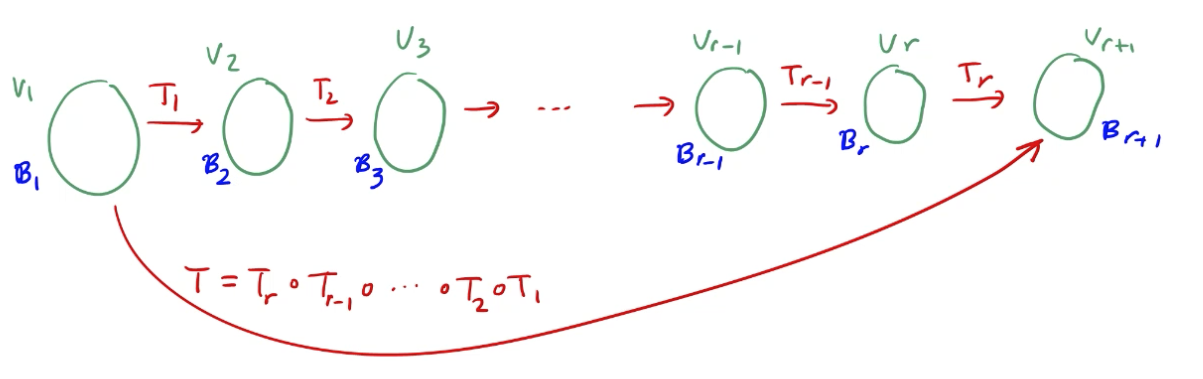
\includegraphics[width=\columnwidth]{images/T2.9.1.png}

\subsection{Matrices for invertible LTs}

\textbf{Theorem 2.10.1.} Let $T: V \mapsto W$ be a linear transformation, $\mathcal{B}$ an ordered basis for $V$ and $\mathcal{B}'$ be an ordered basis for $W$. Then $T$ is an isomorphism iff the matrix $[T]_{\mathcal{B'}, \mathcal{B}}$ is invertible. In this case,

$$
[T^{-1}]_{\mathcal{B}, \mathcal{B'}} = ([T]_{\mathcal{B'}, \mathcal{B}})^{-1}
$$

\textbf{Corollary 2.10.2. (Inverse of matrix of identity operator)} Consider the identity operator $I_V : V \mapsto V$ on $V$ and let $\mathcal{B}$ and $\mathcal{B'}$ be two ordered bases for $V$. Then

$$
[I_V]_{\mathcal{B}, \mathcal{B'}} = ([I_V]_{\mathcal{B'}, \mathcal{B}})^{-1}
$$

\textbf{Remarks.} Forward direction of Theorem 2.10.1. If $\mathcal{B} = \mathcal{B'}$ and $\dim V = n$, then $[I_V]_{\mathcal{B}} = [I_V]_{\mathcal{B}, \mathcal{B}} = I_n$  is the identity matrix. 

\subsection{Change of basis}

\textbf{Theorem 2.11.1.} Let $V$ be a finite dimensional vector space and let $\mathcal{B}$ and $\mathcal{B'}$ be two ordered bases of $V$. Then for any $\mathbf{v} \in V$,

$$
[\mathbf{v}]_{\mathcal{B}} = [I_V]_{\mathcal{B}, \mathcal{B'}} [\mathbf{v}]_{\mathcal{B'}}
$$

Note that $I_V: V \mapsto V$ is the identity linear transformation.

\textbf{Definition.} The matrix $P = [I_V]_{\mathcal{B}, \mathcal{B'}}$ is called the \textit{transition} matrix from $\mathcal{B'}$ to $\mathcal{B}$.

% \textbf{Remarks}

% (i) If $B' = \{ \mathbf{v'_1}, \cdots, \mathbf{v'_n} \}$, then

% $$
% P = ( [\mathbf{v'_1}]_\mathcal{B} \mid \cdots \mid [\mathbf{v'_n}]_\mathcal{B} )
% $$

% (ii) By Corollary 2.10.2, $P$ is invertible and $P^{-1} = [I_V]_{\mathcal{B'}, \mathcal{B}}$.

\textbf{Theorem 2.11.2.} Let $V$ be a finite dimensional vector space and $T: V \mapsto V$ a linear operator on $V$. If $\mathcal{B}$ and $\mathcal{B'}$ are two ordered bases of $V$ and $P = [I_V]_{\mathcal{B}, \mathcal{B'}}$ is the transition matrix from $\mathcal{B'}$ to $\mathcal{B}$, then

$$
[T]_{\mathcal{B'}} = P^{-1} [T]_{\mathcal{B}} P = [I_V]_{\mathcal{B'}, \mathcal{B}} [T]_{\mathcal{B}} [I_V]_{\mathcal{B}, \mathcal{B'}}
$$

\textbf{Definition (similar matrices)} Let $A$ and $B$ be two matrices over the field $\mathbb{F}$. We say $B$ is \textit{similar} to $A$ over $\mathbb{F}$ if there is an invertible $n \times n$ matrix $P$ such that $B = P^{-1} AP$.

\textbf{Definition (determinant of a linear operator)}. If $T: V \mapsto V$ is a linear operator, then the \textit{determinant} of $T$ is the determinant of \textit{any} matrix which represents $T$. More precisely, if $\mathcal{B}$ is an ordered basis of $V$ and $A = [T]_{\mathcal{B}}$ the matrix which represents $T$ wrt $\mathcal{B}$, then

$$
\det T = \det A
$$

\subsection{Chapter 2 Tutorial Theorems}

\textbf{T5Q3.} Let $U$ and $V$ be vector spaces over a field $\mathbb{F}$ and let $T : U \mapsto V$ be a linear transformation. Suppose that $\{ \mathbf{u_1}, \cdots, \mathbf{u_n} \}$ spans $U$.

(a) $\{ T(\mathbf{u_1}), \cdots, T(\mathbf{u_n}) \}$ spans $\mathcal{R}(T)$.

(c) If $T$ is injective and $\{ \mathbf{u_1}, \cdots, \mathbf{u_n} \}$ is a basis for $U$, then $\{ T(\mathbf{u_1}), \cdots, T(\mathbf{u_n}) \}$ is a basis for $\mathcal{R}(T)$.

(e) If $T$ is an isomorphism, then $\{ T(\mathbf{u}_1, \cdots \mathbf{u}_n) \}$ is a basis for $V$ and $\dim U = \dim V$. So an isomorphism sends a basis for U to a basis for V, and finite dimensional vector spaces which are isomorphic to each other have the same dimension.

\textbf{T5Q6.} Let $\mathbb{F}$ be a field. For each $A \in M_{mn}(\mathbb{F})$, let $T_A : \mathbb{F}^n \mapsto \mathbb{F}^m$ be defined by 

$$
T_A(\mathbf{u}) = A\mathbf{u}, \quad \mathbf{u} \in \mathbb{F}^n
$$

(i) $T: \mathbb{F}^n \mapsto \mathbb{F}^M$ is a linear transformation iff there exists $A \in M_{mn}(\mathbb{F})$ such that $T = T_A$.

(ii) If $A, B \in M_n(\mathbb{F})$ and $AB = I$, then $BA = I$. Recall that the inverse of $A$ is the matrix $B$ such that $AB = BA = I$. The above says that to prove that $B$ is the inverse of $A$, we only need to check $AB = I$.

\textbf{T6Q3} Let $V$ and $W$ be finite dimensional vector spaces and $T: V \mapsto W$ a linear transformation. 

(a) If $\dim V < \dim W$, then $T$ is not surjective.

(b) If $\dim V > \dim W$, then $T$ is not injective.

\textbf{T6Q5.} Let $T: V \mapsto V$ be a linear operator such that $T^2 = T$. Such an operator is called a \textbf{projection} of $V$. The direct sum decomposition of $V = \mathcal{R}(T) \oplus \ker (T)$ is equivalent to projections of $V$.

% \textbf{T6Q5} Let $V$ be a finite dimensional vector space. Let $T : V \mapsto V$ be a linear operator such that $T^2 = T$. Such an operator is called a \textbf{projection} of $V$.

% (i) If $\mathbf{v} \in V$, then $\mathbf{v} \in \mathcal{R}(T)$ iff $T(\mathbf{v}) = \mathbf{v})$.

% (ii) $V = \ker(T) \oplus \mathcal{R}(T)$

% (iii) There is an ordered basis $\mathcal{B}$ of $V$ such that

% $$
% [T]_{\mathcal{B}} = 
% \begin{pmatrix}
% I_r & 0 \\
% 0 & 0 \\
% \end{pmatrix}
% $$

% where $r = rank(T)$, $I_r$ is the $r \times r$ identity matrix, and each 0 represents a zero matrix of appropriate size.

% (b) Conversely, let $W_1$ and $W_2$ be two subspaces of $V$ such that $V = W_1 \oplus W_2$. There is a unique projection $T: V \mapsto V$ such that $\mathcal{R}(T) = W_1$ and $\ker(T) = W_2$.

% \textbf{T6Q6} Let $V$ be a finite dimensional vector space and $T: V \mapsto V$ and $S: V \mapsto V$ be linear operators.

% (i) $\ker (T) \subseteq \ker (ST)$.

% (ii) $\mathcal{R} (ST) \subseteq \mathcal{R} (S)$.

% (iii) If $n_T = nullity(T)$ , $n_s = nullity(S)$, and $n_{ST} = nullity(ST)$, then

% $$
% \max (n_T, n_S) \leq n_{ST} \leq n_T + n_S
% $$

% \textbf{T7H1} Let $U$ and $V$ be finite dimensional vector spaces over a field $\mathbb{F}$ and $\dim U < \dim V$, and let $T: U \mapsto V$ and $S: V \mapsto U$ be linear transformations. $T \circ S : V \mapsto V$ is \textbf{not} an isomorphism.

% \textbf{T7Q6 (Converse of Theorem 2.11.2)} Let $V$ be an $n-$dimensional vector space over a field $\mathbb{F}$ and $T: V \mapsto V$ a linear operator. Suppose that $\mathcal{B}$ is a basis for $V$ and $A = [T]_{\mathcal{B}}$. If $P$ is an invertible $n \times n$ matrix over $\mathbb{F}$, then there is a $\mathcal{B}'$ for $V$ such that 

% $$
% [T]_{\mathcal{B'}} = P^{-1}AP
% $$

% \textbf{Definition (Injective).} $T$ is injective if $\forall \mathbf{v_1}, \mathbf{v_2}, \in V$,

% $$
% T(\mathbf{v}_1) = T(\mathbf{v}_2) \implies \mathbf{v}_1 = \mathbf{v}_2.
% $$

% \textbf{Definition (Surjective).} If $T: V \mapsto W$, then $T$ is surjective if

% $$
% \forall w \in W, \exists v \in V, T(v) = w
% $$

% \textbf{Theorem.} 

% (i) If $f \circ g$ is injective, then $g$ is injective.

% (ii) If $f \circ g$ is injective and $g$ is surjective, then both $f$ and $g$ are injective.

\textbf{Theorem.} The composition of injective/surjective/bijective functions is injective/surjective/bijective.

\section{3: Diagonalization and Jordan Canonical Forms}

\textbf{Problem:} Find an ordered basis $\mathcal{B}$ of $V$ such that the matrix $[T]_\mathcal{B}$ of $T$ wrt $\mathcal{B}$ is in an especially simple form.

\subsection{Diagonalizable linear operators.} 

% \textbf{Properties of diagonal matrices.} Suppose a linear operator $T: V \mapsto V$ and an ordered basis $\mathcal{B} = \{ \mathbf{v_1}, \cdots, \mathbf{v_n} \}$ of $V$ are such that $[T]_{\mathcal{B}} = D$.

% $$
% D=\left(\begin{array}{ccccc}
% \lambda_{1} & 0 & 0 & \cdots & 0 \\
% 0 & \lambda_{2} & 0 & \cdots & 0 \\
% \vdots & \vdots & \vdots & \ddots & \vdots \\
% 0 & 0 & 0 & \cdots & \lambda_{n}
% \end{array}\right)
% $$

% The following are immediate:

% (a) $T(\mathbf{v_j}) = \lambda_j \mathbf{v_j}$ for $j = 1, 2, \cdots, n$. (The vectors $\mathbf{v_1, \cdots, v_n}$ are called the \textit{eigenvectors} of $T$.

% (b) Assume that $\lambda_1, \cdots, \lambda_r \neq 0$ and $\lambda_{r+1} = \cdots = \lambda_n = 0$. Then

% $$
% T(c_1 \mathbf{v_1} + \cdots + c_n \mathbf{v_n}) = c_1 \lambda_1 \mathbf{v_1} + \cdots + c_r \lambda_r \mathbf{v}_r
% $$

% It follows that $\mathcal{R}(T) = Span\{ \mathbf{v_1, \cdots, v_r} \}$ and $\ker(T) = Span\{ \mathbf{v_{r+1}, \cdots, v_n} \}$. In particular, $nullity(T)$ is the number of 0 on the diagonal of D.

% (c) $\det(T) = \det(D) = \lambda_1 \lambda_2 \cdots \lambda_n$.

% (d) For any positive integer $k$, the matrix of $T^k$ relative to $\mathcal{B}$ is given by 

% $$
% \left[T^{k}\right]_{\mathcal{B}}=D^{k}=\left(\begin{array}{ccccc}
% \lambda_{1}^{k} & 0 & 0 & \cdots & 0 \\
% 0 & \lambda_{2}^{k} & 0 & \cdots & 0 \\
% 0 & 0 & \lambda_{3}^{k} & \cdots & 0 \\
% \vdots & \vdots & \vdots & \ddots & \vdots \\
% 0 & 0 & 0 & \cdots & \lambda_{n}^{k}
% \end{array}\right) 
% $$

% \textbf{Definition}  A linear operator $T : V \mapsto V$ is called \textit{diagonalizable} if $V$ has an ordered basis $\mathcal{B}$ such that the matrix $[T]_{\mathcal{B}}$ is diagonal.

% \textbf{Definition} Let $V$ be a vector space over a field $\mathbb{F}$ and $T: V \mapsto V$ a linear operator. A scalar $\lambda \in \mathbb{F}$ is called an \textit{eigenvalue} of $T$ if there exists a \textbf{nonzero} vector $\mathbf{v} \in V$ such that

% $$
% T(\mathbf{v}) = \lambda v
% $$

% In this case, $\mathbf{v}$ is called an \textit{eigenvector} of $T$ corresponding to the eigenvalue $\lambda$.

\textbf{Theorem 3.1.1.} A linear operator $T: V \mapsto V$ is diagonalizable iff $V$ has a basis $\mathcal{B}$ such that each of its element is an eigenvector of $T$. In this case, $[T]_{\mathcal{B}}$ is diagonal, and the diagonal entries of $[T]_{\mathcal{B}}$ are the eigenvalues of $T$.

\textbf{Definition}

(i) The polynomial $c_T(x)$ defined by 

$$
c_T(x) = \det (xI - T) = a_0 + a_1x + \cdots + a_{n-1}x^{n-1} + x^n
$$

is called the \textit{characteristic polynomial} of $T$.

(ii) The equation 

$$
c_T(x) = 0
$$

is called the \textit{characteristic equation} of $T$.

(iii) If $\lambda$ is an eigenvalue of the linear operator $T: V \mapsto V$, then the subspace of $V$

$$
E_{\lambda} (T) = \ker (T - \lambda I_V) = \{ \mathbf{v} \in V : T(\mathbf{v}) = \lambda \mathbf{v} \} 
$$

is called the \textit{eigenspace} of $T$ corresponding to the eigenvalue $\lambda$.

\textbf{Fact (T8Q2(b).)} If $c_A(x) = a_0 + a_1x + \cdots a_n x^n$, then $\det A = (-1)^n a_0 = (-1)^n c_A(0)$.

% $$
% \begin{aligned}
% E_{\lambda}(T) &= \{ \text{all eigenvectors of $T$ corresp to eigenvalue $\lambda$} \} \\
% & \cup \{ \mathbf{0} \}
% \end{aligned}
% $$

% $$
% \begin{aligned}
% & T(\alpha_1 \mathbf{v}_1 + \alpha_2 \mathbf{v_2} + \cdots + \alpha_m \mathbf{v_m}) = \\
% & \alpha_1 T(\mathbf{v}_1) + \alpha_2 T(\mathbf{v}_2) + \cdots + \alpha_m T(\mathbf{v}_m)
% \end{aligned}
% $$

% \textbf{Definition (Eigenvalues/vectors of square matrix)} Let $A \in M_n(\mathbb{F})$. Consider the left multiplication transformation $L_A: \mathbb{F}^n \mapsto \mathbb{F}^n$ defined by $L_A(\mathbf{v}) = A \mathbf{v}, \forall \mathbf{v} \in \mathbb{F}^n$.

% (i) We say that $A$ is \textit{diagonalizable} if the linear operator $L_A$ is diagonalizable. Equivalently, $A$ is diagonalizable iff there is an invertible matrix $P$ such that the matrix $P^{-1}AP$ is diagonal.

% (ii) A nonzero vector $\mathbf{v} \in \mathbb{F}^n$ is called an \textit{eigenvector} of $A$ if $\mathbf{v}$ is an eigenvector of $L_A$, i.e. $L_A(\mathbf{v}) = A\mathbf{v} = \lambda \mathbf{v}$ for some $\lambda \in \mathbb{F}$. In this case, $\lambda$ is called an eigenvalue of $A$.

% (iii) The polynomial $c_A(x)$ defined by

% $$
% c_A(x) = \det (xI - A)
% $$

% is called the characteristic polynomial of $A$.

% (iv) If $\lambda$ is an eigenvalue of $A$, then the \textit{eigenspace} of $A$ corresponding to $\lambda$ is the subspace

% $$
% E_{\lambda}(A) = \{ \mathbf{v} \in \mathbb{F}^n : A \mathbf{v} = \lambda \mathbf{v} \}
% $$

% of $\mathbb{F}^n$ (i.e. $E_{\lambda}(A) = E_{\lambda}(L_A)$.) Note that $E_{\lambda}(A)$ is the solution space of the linear system

% $$
% (A - \lambda I)\mathbf{x} = \mathbf{0}
% $$

% Our plan is to transfer the problem of finding eigenvalues and eigenvectors of a linear operator
% to that of its matrix representation.

% \textbf{Finding eigenvalues/vectors of a matrix.} Let $A$ be a $n \times n$ matrix over $\mathbb{F}$.

% (a) To find the eigenvalues of $A$, we solve the characteristic equation

% $$
% c_A(x) = 0
% $$

% (b) To find the eigenvectors corresponding to the eigenvalue $\lambda$, we solve the homogenous linear system (using GJE)

% $$
% (A - \lambda I) \mathbf{x} = \mathbf{0}
% $$

% \textbf{Finding eigenvalues/vectors of a linear operator.} Let $T: V \mapsto V$ be a linear operator and $n = \dim V$. Let $\mathcal{B}$ be an ordered basis of $V$ and $A = [T]_{\mathcal{B}}$ the matrix of $T$ relative to $\mathcal{B}$. Then the matrix of the linear operator $xI - A$ relative to $\mathcal{B}$ is given by

% $$
% [xI_V - T]_{\mathcal{B}} = xI_n - A
% $$

% Thus,

% $$
% c_T(x) = \det(xI_V - T) = \det (xI_n - A) = c_A(x)
% $$

% that is, the characteristic polynomial of $T$ is the same as the characteristic polynomial of any matrix $A$ which represents $T$. It also follows that

% $$
% c_T(\lambda) = 0 \iff c_A(\lambda) = 0
% $$

% that is, $\lambda$ is an eigenvalue of $T$ iff $\lambda$ is an eigenvalue of $A$. Moreover, for $\mathbf{v} \in V$

% $$
% T(\mathbf{v}) = \lambda \mathbf{v} \iff [T(\mathbf{v})]_{\mathcal{B}} = [\lambda \mathbf{v}]_{\mathcal{B}}
% \iff A[v]_{\mathcal{B}} = \lambda [v]_{\mathcal{B}}
% $$

% So, $\mathbf{v}$ is an eigenvector of $T$ iff $[\mathbf{v}]_{\mathcal{B}}$ is an eigenvector of $A$.

% We now recall from Theorem 2.7.1. that the map $\phi : V \mapsto \mathbb{F}^n$ defined by $\phi(\mathbf{v}) = [\mathbf{v}]_{\mathcal{B}}$ for all $\mathbf{v} \in V$ is an isomorphism. Then we have

% $$
% E_{\lambda} (A) = \phi (E_{\lambda}(T)), \text{ and } \dim (E_{\lambda}(A)) = \dim (E_{\lambda}(T))
% $$

% Thus, finding eigenvalues and eigenvectors of $T$ is equivalent to finding eigenvalues and eigenvectors of $A = [T]_{\mathcal{B}}$.

\textbf{Definition} If the leading coefficient of a polynomial $p(x)$ is $1$, that is $p(x)$ is of the form

$$
p(x) = x^n + a_{n-1}x^{n-1} + \cdots + a_1 x + a_0,
$$

then $p(x)$ is called a \textit{monic} polynomial.

\textbf{Theorem 3.1.2.} If $A \in M_n(\mathbb{F})$, then the characteristic polynomial $c_A(x)$ of $A$ is a monic polynomial of degree $n$.

\subsection{Conditions for diagonalizability}

% \textbf{Theorem 3.2.1.} Let $T: V \mapsto V$ be a linear operator. If $\{ \mathbf{v}_1, \cdots, \mathbf{v}_k \}$ is a set of eigenvectors, each corresponds to a distinct eigenvalue, then it is linearly independent.

% \textbf{Corollary 3.2.2.} Let $T: V \mapsto V$ be a linear operator. If $\dim V = n$ and $T$ has $n$ distinct eigenvalues, then $T$ is diagonalizable.

\textbf{Theorem 3.2.3.} Let $T: V \mapsto V$ be a linear operator and let $\lambda_1, \cdots, \lambda_r$ be the distinct eigenvalues of $T$. For each $1 \leq i \leq r$, let $E_{\lambda_i}$ be the eigenspace of $T$ corresponding to $\lambda_i$. The following are equivalent:

(i) $T$ is diagonalizable

(ii) The characteristic polynomial for $T$ is

$$
c_T(x) = (x - \lambda_1)^{d_1} \cdots (x - \lambda_r)^{d_r}
$$

where $\dim E_{\lambda_i} (T) = d_i$ for $i = 1, 2, \cdots, r$.

(iii) $\dim E_{\lambda_1}(T) + \cdots + \dim E_{\lambda_r}(T) = \dim V$.

(iv) $V = E_{\lambda_1}(T) \oplus \cdots \oplus E_{\lambda_r}(T) $

% \textbf{Procedure to determine if a matrix is diagonlizable.} P11 of lecture notes.

\subsection{Invariant subspaces}

\textbf{Definition} Let $T : V \mapsto V$ be a linear operator. A subspace $W$ of $V$ is called a $T$\textbf{-invariant subspace} of $V$ if $T(W) \subseteq W$ (i.e. $T(\mathbf{w}) \in W, \forall \mathbf{w} \in W$).

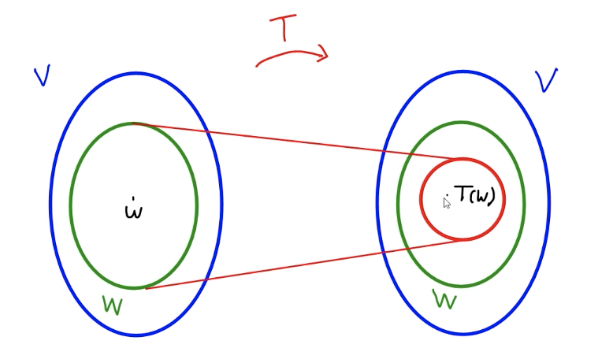
\includegraphics[width=\columnwidth]{images/t-invariant.png}

\textbf{Definition} Let $T: V \mapsto V$ be a linear operator and let $W \subseteq V$ be a $T-$invariant subspace of $V$. Define $T_W : W \mapsto W$ by 

$$
T_W(\mathbf{w}) = T(\mathbf{w}) \quad \forall \mathbf{w} \in W
$$

Then $T_W$ is a linear operator on $W$, called the \textit{restriction of $T$ to $W$}.

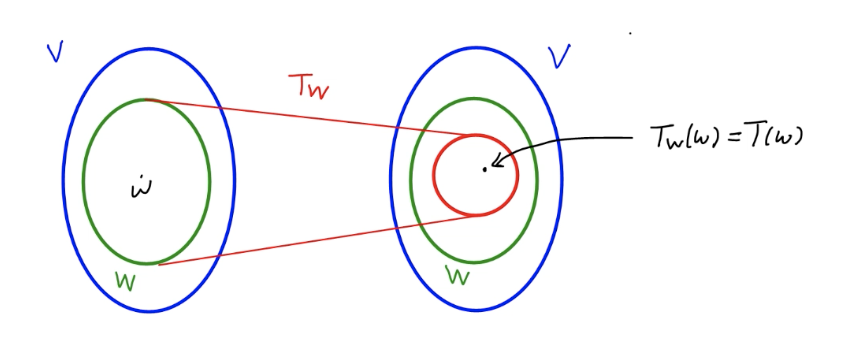
\includegraphics[width=\columnwidth]{images/restriction-t-w.png}

% \textbf{Theorem 3.3.1.} Let $V$ be a finite dimensional vector space. If $T: V \mapsto V$ is a linear operator and $W \subseteq V$ is a $T-$invariant subspace of $V$, then the characteristic polynomial of $T_W$ divides the characteristic polynomial of $T$, that is, $c_T(x) = c_{T_W}(x)q(x)$ for some polynomial $q(x)$.

\textbf{Definition} Let $T: V \mapsto V$ be a linear operator and let $\mathbf{u}$ be a nonzero vector in $V$. The subspace

$$
W = Span\{ \mathbf{u}, T(\mathbf{u}), T^2(\mathbf{u}) \cdots \}
$$

is called the \textit{T-cyclic subspace of V generated by $\mathbf{u}$}. It is a \textit{T-}invariant subspace of $V$.

% \textbf{Theorem 3.3.2.} Let $V$ be a finite dimensional vector space, $T: V \mapsto V$ be a linear operator, $W$ the T-cyclic subspace of $V$ generated by a nonzero vector $\mathbf{u} \in V$ and $m = \dim W$.

% (i) The set $\{ \mathbf{u}, T(\mathbf{u}), T^2(\mathbf{u}) \cdots, T^{m=1}(\mathbf{u}) \}$ is a basis for $W$.

% (ii) There exist scalars $a_0, a_1, \cdots, a_{m-1} \in \mathbb{F}$ such that 

% $$
% a_0 \mathbf{u} + a_1 T(\mathbf{u}) + \cdots + a_{m-1}T^{m-1}(\mathbf{u}) + T^m(\mathbf{u}) = \mathbf{0}
% $$

% and the characteristic polynomial of $T_W$ is given by

% $$
% c_{T_W}(x) = a_0 + a_1x + \cdots + a_{m-1}x^{m-1} + x^m
% $$

\subsection{Cayley-Hamilton Theorem}

\textbf{Remark} If $\mathcal{B}$ is an ordered basis for $V$ and $[T]_{\mathcal{B}} = A$, then 

$$
[f(T)]_{\mathcal{B}} = f(A)
$$

where $f(x) = a_0 + a_1x + \cdots + a_nx^n$ is a polynomial over $\mathbb{F}$. 

\textbf{Cayley Hamilton Theorem.} Let $T$ be a linear operator on a finite-dimensional vector space $V$, and let $c_T(x)$ be the characteristic polynomial of $T$. Then

$$
c_T(T) = T_0
$$

where $T_0$ is the zero transformation. 

% \textbf{Cayley-Hamilton Theorem for Matrices.} Let $A \in M_n(\mathbb{F})$ and let $c_A(x)$ be its characteristic polynomial. Then 

% $$
% c_A(A) = O{nn}
% $$

% is the $n \times n$ zero matrix.

\subsection{Minimal Polynomial}

\textbf{Definition} Let $V$ be a finite dimensional vector space over a field $\mathbb{F}$, and let $T: V \mapsto V$ be a linear operator. A polynomial $m_T(x) \in P(\mathbb{F})$ is called a \textit{minimal polynomial} of $T$ if it has the following properties:

(i) $m_T(x)$ is \textit{monic}.

(ii) $m_T(T) = T_0$.

(iii) If $p(x)$ is a nonzero polynomial and $p(T) = T_0$, then 

$$
\deg (m_T(x)) \leq \deg (p(x))
$$

that is, $m_T(x)$ has the smallest degree among all the nonzero polynomials $p(x)$ with the property $p(T) = T_0$.

\textbf{Theorem 3.5.1.} Let $V$ be a finite dimensional vector space, $T: V \mapsto V$ a linear operator and $m_T(x)$ a minimal polynomial of $T$.

(i) If $p(x)$ is a polynomial such that $p(T) = T_0$, then $m_T(x)$ divides $p(x)$, that is, 

$$
p(x) = q(x) m_T(x)
$$

for some polynomial $q(x) \in P(\mathbb{F})$. In particular, $m_T(x)$ divides $c_T(x)$.

(ii) The minimal polynomial of $T$ is unique.

\textbf{Theorem 3.5.2} Let $V$ be a finite dimensional vector space and let $T: V \mapsto V$ be a linear operator. Then the minimal polynomial $m_T(x)$ of $T$ and the characteristic polynomial $c_T(x)$ of $T$ have the same roots, that is, for any scalar $\lambda$, 
$$
m_T(\lambda) = 0 \iff c_T(\lambda) = 0
$$

Hence, $\lambda$ is an eigenvalue of $T$ iff $m_T(\lambda) = 0$.

\textbf{Theorem 3.5.3.} Let $T: V \mapsto V$ be a linear operator and let $\lambda_1, \cdots, \lambda_k$ be the distinct eigenvalues of $T$. Then $T$ is diagonalizable iff the minimal polynomial of $T$ is the form 

$$
m_T(x) = (x - \lambda_1)(x - \lambda_2) \cdots (x - \lambda_k)
$$

% \textbf{Definition} Let $A \in M_n(\mathbb{F})$. A polynomial $m_A(x) \in P(\mathbb{F})$ is called a \textit{minimal polynomial} of $A$ if it has the following properties:

% (i) $m_A(x)$ is monic.

% (ii) $m_A(A) = 0_{nn}$.

% (iii) If $p(x)$ is a nonzero polynomial and $p(A) = O_{nn}$, then the degree of $m_A(x)$ is less than or equal to the degree of $p(x)$. That is, $m_A(x)$ has the smallest degree among all the nonzero polynomials $p(x)$ with the property $p(A) = O_{nn}$.

% \textbf{Theorem 3.5.4.} Let $A \in M_{n}(\mathbb{F})$ and let $m_A(x)$ be a minimal polynomial of $T$.

% (i) If $p(x)$ is a polynomial such that $p(A) = O_{nn}$, then $m_A(x)$ divides $p(x)$, that is,

% $$
% p(x) = m_A(x)q(x)
% $$

% for some polynomial $q(x) \in P(\mathbb{F})$. In particular, $m_A(x)$ divides $c_A(x)$.

% (ii) The minimal polynomial of $A$ is unique.

% \textbf{Theorem 3.5.5.} Let $T: V \mapsto V$ be a linear operator, $\mathcal{B}$ an ordered basis for $V$ and $A = [T]_{\mathcal{B}}$. Then

% $$
% m_T(x) = m_A(x)
% $$

% \textbf{Corollary 3.5.6.} Let $A \in M_n(\mathbb{F})$.

% (i) Let $L_A: \mathbb{F}^n \mapsto \mathbb{F}^n$ be the left multiplication transformation defined by $L_A(\mathbf{u}) = A \mathbf{u}, \forall \mathbf{u} \in \mathbb{F}^n$. Then 

% $$
% m_A(x) = m_{L_A}(x)
% $$

% (ii) For any scalar $\lambda$, $m_A(\lambda) = 0$ iff $c_A(\lambda) = 0$.

% (iii) If $\lambda_1, \cdots, \lambda_k$ are the distinct eigenvalues of $A$, then $A$ is diagonalizable iff

% $$
% m_A(x) = (x - \lambda_1)(x - \lambda_2) \cdots (x - \lambda_k)
% $$

\subsection{Generalized Eigenspace}
Throughout this section, assume that (i) $\mathbb{F} = \mathbb{C}$, (ii) $V$ is a finite dimensional \textbf{complex} vector space and (iii) $T : V \mapsto V$ is a linear operator.

\textbf{Fundamental Theorem of Algebra.} The characteristic polynomial of $T$ can be factorized as 

$$
c_T(x) = (x - \lambda_1)^{m_1} (x - \lambda_2)^{m_2} \cdots (x - \lambda_k)^{m_k}
$$

For each $1 \leq i \leq k$, we call the positive integer $m_i$ the \textbf{multiplicity} of the eigenvalue $\lambda_i$.

\textbf{Definition} Let $\lambda \in \mathbb{C}$. A nonzero vector $\mathbf{v} \in V$  is called a \textbf{generalized eigenvector} of $T$ corresponding to $\lambda$ if there exists a positive integer $m$ such that

$$
(T - \lambda I_V)^m (\mathbf{v}) = \mathbf{0}
$$

Every eigenvector of $T$ is a generalized eigenvector of $T$ . However, a generalized eigenvector of $T$ may not be an eigenvector of $T$ .

\textbf{Theorem 3.6.1} If $\mathbf{v}$ is a generalized eigenvector of $T$ corresponding to $\lambda$, then $\lambda$ is an eigenvalue of $T$.

\textbf{Definition} Let $\lambda$ be an eigenvalue of $T: V \mapsto V$. THe subset $K_{\lambda}(T)$ of $V$ defined by

$$
\begin{aligned}
K_{\lambda}(T) &= \{ \mathbf{v} \in V: (T - \lambda I_V)^m (\mathbf{v}) = \mathbf{0} \\ 
&\text{ for some positive integer $m$ }   \}
\end{aligned}
$$

is called \textbf{the generalized eigenspace of $T$ corresponding to $\lambda$}.

\textbf{Theorem 3.6.2.} If $\lambda$ be an eigenvalue of $T$, then the generalized eigenspace $K_{\lambda}(T)$ is a $T-$invariant subspace of $V$.

\textbf{Theorem 3.6.3.} Let $T: V \mapsto V$ be a linear operator and let $\lambda_1, \cdots, \lambda_k$ be the distinct eigenvalues of $T$. Then

$$
V = K_{\lambda_1}(T) \oplus K_{\lambda_2}(T) \cdots \oplus K_{\lambda_k}(T)
$$

\textbf{Theorem 3.6.4.} Let $\lambda$ be an eigenvalue of $T$ with multiplicity $m$.

(i) $E_{\lambda}(T) \subseteq K_{\lambda}(T)$.

(ii) If $\mu \in \mathbb{C}$ and $\mu \neq \lambda$, then $E_{\mu} (T) \cap K_{\lambda}(T) = \{ \mathbf{0} \}$.

(iii) If $\mu \in \mathbb{C}$ and $\mu \neq \lambda$, then the restriction of $T - \mu I_V$ to $K_{\lambda}(T)$ is injective and

$$
(T - \mu I_V)(K_{\lambda}(T)) = K_{\lambda}(T)
$$

(iv) $\dim K_{\lambda}(T) \leq m$. Remark: Proved later that $\dim K_{\lambda}(T) = m$.

(v) $K_{\lambda}(T) = Ker(T - \lambda I_V)^m$ (m is fixed)

% \textbf{Theorem 3.6.5.} Let $T: V \mapsto V$ be a linear operator and let $\lambda_1, \cdots, \lambda_k$ be the distinct eigenvalues of $T$. Then 

% $V = K_{\lambda_1}(T) + K_{\lambda_2}(T) + \cdots + K_{\lambda_k}(T)$.

% \subsection{Chapter 3 Tutorial Theorems}

% \textbf{T8Q2} Let $A$ be a $n \times n$ matrix over a field $\mathbb{F}$.

% (a) If $\lambda$ is an eigenvalue of $A$, then $\lambda^k$ is an eigenvalue of $A^k$ for any positive integer $k$.

% (b) If $c_A(x) = a_0 + \cdots + a_nx^n$, then $\det A = (-1)^n a_0 = (-1)^n c_A (0)$.

% (c) $A$ is invertible iff $0$ is not an eigenvalue of $A$.

% (d) If $A$ is invertible, then $\lambda$ is an eigenvalue of $A$ iff $\frac{1}{\lambda}$ is an eigenvalue of $A^{-1}$.

% (e) If $A$ and $B$ are similar, that is, $B = P^{-1}AP$ for some matrix $P$, then $c_A(x) = c_B(x)$.

\subsection{Jordan Canonical Form}
Throughout this section, assume that (i) $\mathbb{F} = \mathbb{C}$, (ii) $V$ is a finite dimensional \textbf{complex} vector space and (iii) $T : V \mapsto V$ is a linear operator.

\textbf{Definition} Let $\mathbf{v} \in V$ be a generalized eigenvector of $T$ corresponding to the eigenvalue $\lambda$, and let $p$ be the smallest positive integer such that $(T - \lambda I_V)^p (\mathbf{v}) = \mathbf{0}$. Then the ordered set of vectors

$$
C=\left\{\left(T-\lambda I_{V}\right)^{p-1}(\mathbf{v}), \ldots,\left(T-\lambda I_{V}\right)(\mathbf{v}), \mathbf{v}\right\}
$$

is called \textbf{a cycle of generalized eigenvectors of $T$ corresponding to $\lambda$}.

(i) The vector $(T - \lambda I_V)^{p - 1} (\mathbf{v})$ is called the \textbf{initial vector} of the cycle. It is the only eigenvector in the cycle.

(ii) The vector $\mathbf{v}$ is called the \textbf{end vector} of the cycle.

(iii) The number of vectors $p$ in the cycle is called the \textbf{length of the cycle.}

\textbf{Observation.} If $C=\left\{\left(T-\lambda I_{V}\right)^{p-1}(\mathbf{v}),\left(T-\lambda I_{V}\right)^{p-2}(\mathbf{v}), \ldots,\left(T-\lambda I_{V}\right)(\mathbf{v}), \mathbf{v}\right\}$ is a cycle of generalized eigenvectors of $T$ corresponding to $\lambda$ and $\mathbf{u} \in C$, then for any positive integer $m$,

$(T - \lambda I_V)^m (\mathbf{u}) = \mathbf{0} \text{ or } \in C$.

% \textbf{Theorem 3.7.1.} Let $T: V \mapsto V$ be a linear operator and let $\lambda$ be an eigenvalue of $T$. Suppose that $C_1, \cdots, C_r$ are cycles of generalized eigenvectors of $T$ corresponding to $\lambda$ such that the initial vectors of the $C_i$'s are distinct and form a linearly independent set. Then:

% (i) The $C_i$'s are disjoint, i.e. $C_i \cap C_j = \emptyset$ whenever $i \neq j$.

% (ii) The union 

% $$
% C = \bigcup^r_{i = 1} C_i
% $$

% is linearly independent.

% \textbf{Corollary 3.7.2.} Every cycle of generalized eigenvectors of a linear operator on $V$ is linearly independent.

\textbf{Theorem 3.7.3.} Let $T : V \mapsto V$ be a linear operator and let $\lambda$ be an eigenvalue of $T$. Then $K_{\lambda}(T)$ has a basis consisting of a union of disjoint cycles of generalized eigenvectors of $T$ corresponding to $\lambda$.

\textbf{Theorem 3.7.4.} Let $T: V \mapsto V$ be a linear operator. Then $V$ has a basis $\mathcal{B}$ such that $\mathcal{B}$ is a disjoint union of cycles of generalized eigenvectors of $T$.

\textbf{Jordan Block} The matrix $J_p(\lambda)$ is called a \textbf{Jordan block} of order $p$ corresponding to $\lambda$.

$$
J_{1}(\lambda)=(\lambda), \quad J_{2}(\lambda)=\left(\begin{array}{cc}
\lambda & 1 \\
0 & \lambda
\end{array}\right)
$$

\textbf{Theorem 3.7.5.} Let $T: V \mapsto V$ be a linear operator. Then V has a Jordan canonical basis $\mathcal{B}$, that is, the matrix $[T]_{\mathcal{B}}$ of $T$ relative to $\mathcal{B}$ is of the form

$$
[T]_{\mathcal{B}}=\left(\begin{array}{cccc}
J_{p_{1}}\left(\lambda_{1}\right) & 0 & \cdots & 0 \\
0 & J_{p_{2}}\left(\lambda_{2}\right) & \cdots & 0 \\
\vdots & \vdots & \ddots & \vdots \\
\mathbf{0} & \mathbf{0} & \cdots & J_{p_{r}}\left(\lambda_{r}\right)
\end{array}\right)
$$

Moreover, the Jordan blocks $J_{p1}(\lambda_1), \cdots, J_{p_r}(\lambda_r)$ are unique up to re-ordering.

\textbf{Remark}

1. The theorem says that the Jordan canonical form of a linear operator $T$ is essentially unique. If we have found one JCF of $T$ , then all other JCFs of $T$ are obtained simply by rearranging the Jordan blocks. They are the matrices of $T$ relative to bases obtained by reordering the elements of $B$.

2. Since the JCF of T is unique up to the reordering of its Jordan blocks, we may call any of the JFCs of T the Jordan canonical form of T .

3. We have proved that a Jordan canonical basis exists. For a proof for the uniqueness of the Jordan blocks, see Section 7.2 of [FIS].

\textbf{Remark} A linear operator $T$ is diagonlizable iff all the jordan blocks in its Jordan canonical form are of order 1, that is, 
$$
\begin{aligned}
[T]_{\mathcal{B}}&=\left(\begin{array}{ccccc}
J_{1}\left(\lambda_{1}\right) & 0 & \cdots & 0 & 0 \\
0 & J_{1}\left(\lambda_{2}\right) & \cdots & 0 & 0 \\
\vdots & \vdots & & \vdots & \vdots \\
0 & 0 & \cdots & J_{1}\left(\lambda_{r-1}\right) & 0 \\
0 & 0 & \cdots & 0 & J_{1}\left(\lambda_{r}\right) \\
\end{array}\right) \\
&=\left(\begin{array}{ccccc}
\lambda_{1} & 0 & \cdots & 0 & 0 \\
0 & \lambda_{2} & \cdots & 0 & 0 \\
\vdots & \vdots & & \vdots & \vdots \\
0 & 0 & \cdots & \lambda_{r-1} & 0 \\
0 & 0 & \cdots & 0 & \lambda_{r}
\end{array}\right)
\end{aligned}
$$

\textbf{Definition.} Let $A \in M_n(\mathbb{C})$. Then the Jordan canonical form of $A$ is defined to be the Jordan canonical form of the linear operator $L_A: \mathbb{C}^n \mapsto \mathbb{C}^n$.

\textbf{Characteristic polynomial.} The characteristic polynomial of $T$ is given by $c_T(x) = c_J(x) = (x - \lambda_1)^{k_1} (x - \lambda_2)^{k_2} \cdots (x - \lambda_r)^{k_r}$.

\textbf{The minimal polynomial of a matrix in Jordan canonical form.}

\textbf{Theorem 3.7.6.} Let $T: V \mapsto V$ be a linear operator and let $J$ be a Jordan canonical form of $T$. Suppose that $\lambda_1, \cdots, \lambda_k$ are the distinct eigenvalues of $T$, and for each $1 \leq i \leq k$, \textbf{$p_i$ is the order of the largest Jordan block corresponding to $\lambda_i$ in $J$.} Then the minimal polynomial of $T$ is given by 

$$
m_T(x) = (x - \lambda_1)^{p_1} (x - \lambda_2)^{p_2} \cdots (x - \lambda_k)^{p_k}
$$

\textbf{Fact.} If the eigenspace $E_{\lambda}(A)$ of $A$ corresponding to the eigenvalue $\lambda$ has dimension $k$, then the number of Jordan blocks corresponding to $\lambda$ in the JCF of $A$ is also $k$.

\section{4: Inner Product Spaces}

\subsection{Inner Product}

% \textbf{Definition} Let $\mathbb{F} = \mathbb{R} or \mathbb{C}$ and let $V$ be a vector space over $\mathbb{F}$. An \textit{inner product} on $V$ is a function which assigns to each ordered pair of vectors $(\mathbf{u}, \mathbf{v})$ in $V$ a scalar $\langle \mathbf{u}, \mathbf{v} \rangle$, and it satisfies the following conditions:

\textbf{Conditions.}

(IP1) $\langle \mathbf{u}, \mathbf{v} \rangle = \overline{\langle \mathbf{v}, \mathbf{u} \rangle}, \forall \mathbf{u, v} \in V$

(IP2+IP3) (linear in the first variable) $\langle \alpha \mathbf{u} + \beta \mathbf{v}, \mathbf{w} \rangle = \alpha \langle \mathbf{u, w} \rangle + \beta \langle \mathbf{v, w} \rangle$ 

(IP4) $\langle \mathbf{v, v} \rangle > 0$ for all nonzero $\mathbf{v} \in V$, and $\langle \mathbf{0, 0} \rangle = 0$.

\textbf{Remarks} 

1. (conjugate linear in the second variable) $\langle \mathbf{w}, \alpha \mathbf{u} + \beta \mathbf{v} \rangle = \bar{\alpha} \langle \mathbf{w, u} \rangle + \bar{\beta} \langle \mathbf{w, v} \rangle$

2. $\langle v, x \rangle = \langle v, y \rangle, \forall v \in V \implies x = y$.

% \textbf{Definition} An \textit{inner product space} is a real or complex vector space $V$ together with an inner product $\langle \cdot, \cdot \rangle$ on $V$.

\textbf{Definition} Let $A \in M_n(\mathbb{C})$. The \textit{conjugate transpose} of $A$ is the matrix $A^* = \bar{A^T}$.

\subsection{Properties of Conjugates}
(i) $|z| = \sqrt{a^2 + b^2} = |\bar{z}|$

(ii) $\bar{z} z = |z|^2$

(iii) $\overline{z_1 + z_2} = \bar{z_1} + \bar{z_2}$

(iv) $\overline{z_1 \times z_2} = \bar{z_1} \times \bar{z_2} $

\subsection{Norm and Distance}

(a) (\textit{norm}) $||\mathbf{u}|| = \sqrt{\langle \mathbf{u, u} \rangle}$

(b) (\textit{distance}) $d(\mathbf{u, v}) = || \mathbf{u - v} ||$.

\textbf{Cauchy-Schwarz Inequality.} If $\mathbf{u, v}$ are two vectors in an inner product space $V$, then 

$$
| \langle \mathbf{u, v} \rangle | \leq || \mathbf{u} || || \mathbf{v} ||
$$

Equality holds iff $\mathbf{u} = c \mathbf{v}$ for some scalar $c$.

\textbf{Triangle Inequality.} If $\mathbf{u, v}$ are two vectors in an inner product space $V$, then

$$
|| \mathbf{u} + \mathbf{v} || \leq || \mathbf{u} || + || \mathbf{v} ||
$$

\subsection{Orthogonal Sets}

\textbf{The Pythagoras Theorem} If $\mathbf{u, v}$ are orthogonal vectors in a inner product space $V$, then

$$
|| \mathbf{u + v} ||^2 = || \mathbf{u} ||^2 + || \mathbf{v} ||^2
$$

\textbf{Theorem 4.4.1} An orthogonal set of nonzero vectors is linearly independent.

% \textbf{Corollary 4.4.2} If $V$ is a finite dimensional inner product space and $n = \dim V$, then any orthogonal set of nonzero vectors in $V$ is finite and contains at most $n$ vectors.

\textbf{Lemma 4.5.1.} Let $\mathcal{B} = \{ \mathbf{v_1, \cdots, v_n} \}$ be an orthonormal basis of $V$. Then for any $\mathbf{v} \in V,$

$$
\mathbf{v}=\left\langle\mathbf{v}, \mathbf{v}_{1}\right\rangle \mathbf{v}_{1}+\left\langle\mathbf{v}, \mathbf{v}_{2}\right\rangle \mathbf{v}_{2}+\cdots+\left\langle\mathbf{v}, \mathbf{v}_{n}\right\rangle \mathbf{v}_{n}
$$

\textbf{Corollary 4.5.2. (Matrix of a linear operator relative to an orthonormal basis)} Let $\mathcal{B} = \{ \mathbf{v_1, \cdots, v_n} \}$ be an orthonormal basis of $V$, $T: V \mapsto V$ a linear operator and $[T]_{\mathcal{B}} = (a_{ij})$. Then for all $i, j$,

$$
a_{ij} = \langle T(\mathbf{v}_j), \mathbf{v}_i \rangle
$$

\textbf{Gram-Schmidt Orthogonalization Process.}

Step 1: Choose $\mathbf{v_1} = \frac{1}{|| \mathbf{u_1} ||} \mathbf{u}_1$

Step 2: Let $\mathbf{v}'_2 = \mathbf{u}_2 - \langle \mathbf{u}_2, \mathbf{v}_1 \rangle \mathbf{v}_1$. Then normalise $\mathbf{v}'$.

Step 3:  Let $
\mathbf{v}_{k+1}^{\prime}=\mathbf{u}_{k+1}-\sum_{j=1}^{n}\left\langle\mathbf{u}_{k+1}, \mathbf{v}_{j}\right\rangle \mathbf{v}_{j}
$. Then normalise $\mathbf{v}_{k+1}$

Step 4: Repeat until we obtain an orthonormal basis $\{ \mathbf{v_1}, \cdots, \mathbf{v_n} \}$ of $V$.

\textbf{Theorem 4.5.3.} Every finite dimensional inner product space has an orthonormal basis

\subsection{Orthogonal Complement}

\textbf{Definition} Let $V$ be an inner product space and $W$ a subspace of $V$. The \textit{orthogonal complement} of $W$ is the set

$$
W^{\perp} = \{ \mathbf{v} \in V: \langle \mathbf{v, w} \rangle = 0, \forall \mathbf{w} \in W \}.
$$

\textbf{Lemma 4.6.1.} If $W$ is a subspace of an inner product space $V$, then its orthogonal complement $W^{\perp}$ is a subspace of $V$. In addition, we have 

$$
W \cap W^{\perp} = \{ \mathbf{0} \}
$$

\textbf{Theorem 4.6.2.} If $W$ is a finite dimensional subspace of an inner product space $V$, then 

$$
V = W \oplus W^{\perp}
$$

\textbf{Remark.} This theorem is false without the assumption that $W$ is finite dimensional.

\subsection{Orthogonal Projections}

% \textbf{Definition} Let $W$ be a finite dimensional subspace of an inner product space $V$. We define the linear operator \textbf{proj}\textsubscript{$W$}$: V \mapsto V$ as follows: by theorem 4.6.2, $V = W \oplus W^{\perp}$. So, for each $\mathbf{v} \in V$, there exist unique vectors $\mathbf{w} \in W$ and $\mathbf{w'} \in W^{\perp}$ such that 

% $$
% \mathbf{v = w + w'} 
% $$

% We set 

\textbf{Definition} The linear operator $proj_W$ is called the orthogonal projection of $V$ on $W$.

$$
proj_W(\mathbf{v}) = \mathbf{w} = \mathbf{v - w'}
$$


\textbf{Remarks}

(b) If $\{ \mathbf{w_1, \cdots, w_k} \}$ is an orthonormal basis of $W$, then 

$$
proj_W(\mathbf{v}) = \sum^k_{j = 1} \langle \mathbf{v, w_j} \rangle \mathbf{w_j}
$$

(c) If $V$ is finite dimensional, then so is $W^{\perp}$. In this case,

$$
proj_{W^{\perp}} (\mathbf{v}) = \mathbf{w'} = \mathbf{v - w} = (I_V - proj_W)(\mathbf{v}), \forall \mathbf{v} \in V
$$

\textbf{Theorem 4.8.1 (Best Approximation)} If $W$ is a finite dimensional subspace of an inner product space $V$ and $\mathbf{v} \in V$, then 

$$
|| proj_{W^{\perp}} (\mathbf{v})  || = || \mathbf{v} - proj_W(\mathbf{v}) || < || \mathbf{v} - \mathbf{w}||
$$

for every vector $\mathbf{w} \in W$ different from $proj_W(\mathbf{v})$.

\textbf{Theorem 4.9.1 (Least Square Solution)} For any real linear system $A \mathbf{x} = \mathbf{b}$, the associated normal system 

$$
(A^tA)\mathbf{x} = A^t \mathbf{b}
$$

is consistent, and all its solutions are least square solutions of $A \mathbf{x} = \mathbf{b}$.

\subsection{The Adjoint of a Linear Operator}

% \textbf{Lemma 4.10.1} Let $V$ be a finite dimensional inner product space over $\mathbb{F}$. If $f: V \mapsto \mathbb{F}$ is a linear functional, then there exists a unique vector $\mathbf{u} \in V$ such that

% $$
% f(\mathbf{v}) = \langle \mathbf{v, u} \rangle, \forall v \in V
% $$

\textbf{Theorem 4.10.2. (adjoint of a linear operator)} Let $T: V \mapsto V$ be a linear operator on a finite dimensional inner product space $V$. Then there exists a unique linear operator $T^*: V \mapsto V$ such that

$$
\langle T(\mathbf{u}), \mathbf{v}) \rangle = \langle \mathbf{u}, T^*(\mathbf{v}) \rangle, \forall \mathbf{u, v} \in V
$$

The operator $T^*$ is called the adjoint of $T$. Generally, adjoint takes the form $(Ax, y) = (x, By)$.

\textbf{Theorem 4.10.3. (Matrix of the adjoint is the conjugate transpose of the matrix)} Let $T: V \mapsto V$ be a linear operator on a finite dimensional inner product space V and $\mathcal{B}$ be an orthonormal basis of $V$. Then

$$
[T^*]_{\mathcal{B}} = ([T]_{\mathcal{B}})^*
$$

\textbf{Lemma 4.10.4.} Let $T, T_1, T_2$ be linear operators on a finite dimensional inner product space $V$. Then:

(i) $(T_1 + T_2)^* = T^*_1 + T^*_2$.

(ii) $(cT)^* = \bar{c}T^*$.

(iii) $(T_1T_2)^* = T^*_2 T^*_1$

(iv) $(T^*)^* = T$.

\subsection{Normal and Self-adjoint operators}

A linear operator $T: V \mapsto V$ is \textbf{orthogonally diagonalizable} if $V$ has an 1) orthonormal basis that 2) consists of eigenvectors of $T$.

\textbf{Definition (self-adjoint)} A linear operator $T: V \mapsto V$ on a finite dimensional inner product space $V$ is called \textit{self-adjoint} if
$$
T = T^*
$$

\textbf{Lemma 4.11.1} All eigenvalues of a self-adjoint operator on a finite dimensional \textit{complex} vector space are real.

\textbf{Corollary 4.11.2} A self-adjoint operator on a finite dimensional real inner product space has at least one eigenvalue.

\textbf{Theorem 4.11.3} A linear operator on a finite dimensional \textit{real} inner product space is orthogonally diagonalizable iff it is self-adjoint.

\textbf{Definition (normal)} A linear operator $T$ on a finite dimensional inner product space is called \textit{normal} if 

$$
TT^* = T^*T
$$

\textbf{Remark.} All self-adjoint operators are normal. Converse is not true.

% \textbf{Theorem 4.11.4.} A linear operator on a finite dimensional \textit{complex} inner product space is orthogonally diagonalizable iff it is normal.

\textbf{Theorem 4.11.4} Let $T: V \mapsto V$ be a linear operator on a finite dimensional complex inner product space. $T$ is a normal operator iff $T$ is orthogonally diagonalizable 

% (iii) (norm of the operator equals the norm of it's adjoint) $|| T(\mathbf{v}) ||  = || T^*(\mathbf{v}) ||$ (T11Q6)

% (iv) $T - \lambda_v$ is normal for every $\lambda \in \mathbb{C}$ (T11Q6)

\textbf{T11Q6} $T(\mathbf{v}) = \lambda \mathbf{v} \implies T^*(\mathbf{v}) = \bar{\lambda} \mathbf{v}, \forall \mathbf{v} \in V$ (T11Q6)

\subsection{Unitary Operators}

\textbf{Definition (Unitary Operator).} A linear operator $T: V \mapsto V$ on a finite dimensional inner product space $V$ is called \textit{unitary} if 

$$
TT^* = T^*T = I_V
$$

that is, $T$ is invertible and $T^{-1} = T^*$.

\textbf{Lemma 4.12.1.} Let $T: V \mapsto V$ be a linear operator on a finite dimensional inner product space $V$. Then the following are equivalent:

(i) $T$ is unitary;

(ii) (Unitary operator preserves inner product) $\langle T(\mathbf{u}), T(\mathbf{v}) \rangle = \langle \mathbf{u, v} \rangle, \forall \mathbf{u, v} \in V$

(iii) $T$ sends an orthonormal basis of $V$ to an orthonormal basis

(iv) (Linear isometry) $|| T(\mathbf{v}) || = || \mathbf{v} ||, \forall v \in V$

% (v) $|\lambda| = 1$, where $\lambda$ is any eigenvalue of $T$. (T11Q5)

\textbf{Remarks.} 

(i) A unitary operator on a complex inner product space is orthogonally diagonalizable because it is normal.

(ii) A unitary operator on a real inner product space need not be orthogonally diagonalizable (as a normal operator need not be self-adjoint.)

% \textbf{Matrix of a unitary operator.} Let $A = [T]_{\mathcal{B}}$.

% $$
% AA^* = A^*A = I_n
% $$

\textbf{Definition. (orthogonal and unitary matrix)}

(Orthogonal) $AA^t = A^tA = I_n$ 

(Unitary) $AA^* = A^*A = I_n$

\textbf{Lemma 4.12.2.} Let $T: V \mapsto V$ be a unitary operator on a finite dimensional inner product space $V$ over $\mathbb{F}$. Let $\mathcal{B}$ be an orthonormal basis of $V$ and let 

$$
A = [T]_{\mathcal{B}}
$$

(i) If $\mathbb{F} = \mathbb{R}$, then $A$ is a real orthogonal matrix.

(ii) If $\mathbb{F} = \mathbb{C}$ then $A$ is a unitary matrix.

\textbf{Columns/Rows of an orthogonal/unitary matrix.} $A$ is an orthogonal/unitary matrix $\iff$ the rows/columns of $A$ form an orthonormal basis of $\mathbb{R}^n/\mathbb{C}^n$.

\textbf{Orthogonally/Unitarily diagonalizable matrices.} 

(Real) $A \in M_n(\mathbb{R})$ is orthogonally diagonalizable iff $A$ is symmetric.

(Complex) $A \in M_n(\mathbb{C})$ is unitarily diagonalizable iff $\exists$ unitary matrix $P$ st $P^*AP$ is diagonal iff $A$ is normal.

\section{Appendix}
\subsection{Properties of Norms}

(i) (Relation between sum of squared norm and squared norm of sum) $|| \sum^n_{i = 1} x_i ||^2 = \sum^n_{i = 1} || x_i ||^2 + \sum_{i \neq j} \langle x_i, x_j \rangle$.

% \subsection{Inverse of matrix}

% (i) For $A = \begin{bmatrix}
% a & b\\
% c & d
% \end{bmatrix}$, 

% $$
% A^{-1} = \frac{1}{\det A} 
% \begin{bmatrix}
% d & -b\\
% -c & a 
% \end{bmatrix}
% $$


% (iii) For $A \in M_{n}(\mathbb{F})$,

% $$
% A^{-1} = \frac{1}{\det A} adj (A)
% $$

% 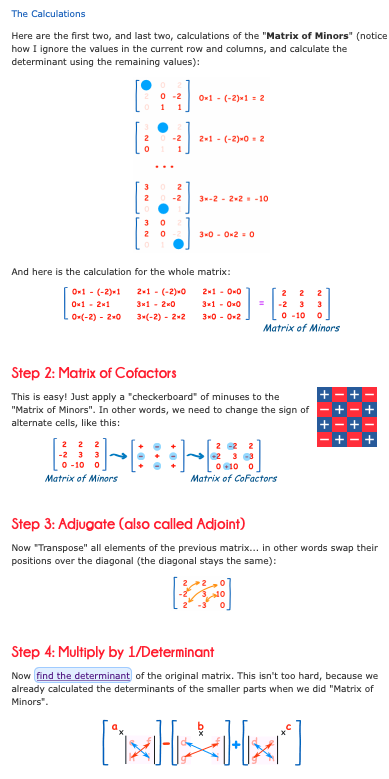
\includegraphics[width=\columnwidth]{images/inverse-matrix.png}

\subsection{List of Questions}
\textbf{Chapter 1}

State matrix multiplication properties

State direct sum of subspaces theorem

State equivalent statements of A is invertible

How to show that a subspace is subset of another subspace with only a set of vectors?

State condition for a subspace to be equal its superspace.

State relationship between summation of dimension of vector spaces and dimension of summation

State multilinear, alternating properties.

$D(X') = ?$

Determinant of lower or upper triangular matrix?

$
\operatorname{det} 
\begin{pmatrix}
A & B \\
0 & C 
\end{pmatrix} = ?
$

If $c_A(x) = a_0 + a_1x + \cdots + x^n, \det(A) = ?$

$\det(AB) = ?$

$\det(A^T) = ?$

$\det(A^{-1}) = ?$

$\det(cA) = ?$

\textbf{Chapter 2}

\textbf{State definition of linear transformation}

State unique linear transformation theorem

State definition of kernel, range, rank, nullity.

State conditions of surjective (1) and injective (1) and bijective (1)

State dimension theorem and it's useful construction of basis.

State relation between $\mathcal{L}(V, W)$ and $V, W$.

State isomorphism definition and properties (2).

State implication of vector spaces which are isomorphic

State $[\mathbf{v}]_{\mathcal{B}}$ naming.

(i) $[\mathbf{v}]_{\mathcal{B}_s} = ?$.

(ii) $[L_M]_{\mathcal{B}_s} = ?$

(iii) $[cT]_{\mathcal{B}} = ?$

(iv) $[T^n]_{\mathcal{B}} = ?$

(v) $[ST]_{\mathcal{B}} = ?$

State $[T]_{B', B}$ naming and decomposition and $[T(v)]_{B'}$ decomposition

State relation between isomorphism and ordered basis

State matrices for composition of LTs

How to check if a linear transformation is an isomorphism from its matrix representation?

How do I easily obtain the inverse of matrix of identity operator?

State change of basis for coordinate matrix and linear transformation.

State composition of injective and surjective functions.

% State conditions for $T: V \mapsto W$ to \textbf{not} be injective or surjective

State relation between projections and direct sum decomposition.

Let $T: V \mapsto W$. 

(i) If $\dim V < \dim W$, what can you say about $T$?

(ii) If $\dim V > \dim W$, what can you say about $T?$

\textbf{Chapter 3}

State diagonalizable implication with basis

State characteristic equation, polynomial and eigenspace definition.

State conditions for diagonalizability

State definition of invariant subspaces and restriction.

How is the linear operator $f(T)$ related to the matrix $f(A)$?

State Cayley Hamilton theorem

\textbf{State minimal polynomial definition}

\textbf{State theorems which relate minimal polynomial with characteristic polynomial (2)}

\textbf{State theorem which relates minimal polynomial and diagonalizable}

\textbf{State definition of generalized eigenvector and eigenspace}

State fundamental theorem of algebra

State how to decompose $V$ to generalised eigenspaces.

State general properties of generalised eigenspace

Define cycle of generalised eigenvectors of T and properties.

Explain how JCF is constructed.

State general fact relating $\dim E_{\lambda}(A)$ and JCF of $A$.

\textbf{Chapter 4}

State conditions for inner product

State properties of Conjugates

Define normal and distance

State Cauchy-Schwarz Inequality

State triangle inequality

State pythagoras theorem

State property of an orthogonal set of nonzero vectors

How to express a vector $\mathbf{v}$ as the linear combination of orthogonal basis vectors?

State matrix of a linear operator relative to an orthonormal basis.

State purpose of Gram-Schmidt Orthogonalization Process

State orthogonal complement definition

State relation between $W^{\perp}$ and $W$. (2)

State definition of projection and how to compute it.

State best approximation and least square solution definition and problem statement.

State adjoint of linear operator and property.

$[T^*]_{\mathcal{B}} = ?$

State general fact of inner product.

State properties of adjoint operators

State definition of orthogonally diagonalizable

State self-adjoint definition and property (1).

State normal definitions definition and properties.

State relation between self-adjoint and normal.

State definition of unitary operator

State properties of unitary operators and conditions of the operator being orthogonally diagonalizable.

State definitions of orthogonal and unitary matrix.

State properties of columns/rows or orthogonal/unitary matrix

$|| \sum^n_{i = 1} x_i ||^2 = ?$.

$(T-S)T = ?$

How to show that 2 vector spaces are equal to one another? (3)

% State conditions for othrogonally/unitarily diagonalizable matrices


\subsection{Exercises}
P29 eg, P30 eg, 1.13.2 proof, T1Q1, T1Q2(a, b), T1Q4 (optional), T1Q6(i, ii), T1Q7, T2H2, T2Q1, T2Q3(c, d, f, g), T2Q4(i (opt), ii, iii), T2Q5, T3Q1(b), T3Q3, T3Q4, T3Q7, T4H1(iii), T4H3(i), T4Q1, T4Q2(ii), T4Q3(c), T4Q5,

\vfill
\hrule
~\\
Prepared by Larry, AY2020/2021 Semester 1
\end{multicols}

\end{document}